\chapter{Denoising}\label{chap:denoising}

Denoising refers to the process of removing unwanted noise from a signal while still retaining its most meaningful components. In the context of underwater acoustic spectrograms, this involves isolating ship radiated noise or narrowband events from background noise such as wind, waves, or marine life. In this chapter we aim to experiment with applying various image denoising methods to underwater acoustic data.

\section{Introduction}

The primary objective of denoising is to recover an underlying clean signal $y$ from its observed noisy recording $x$. Mathematically, the observed signal can be expressed as:
\begin{equation}
    x = y + n
\end{equation}
where $n$ represents the noise contaminating the signal. Recovering $y$ from $x$ is a challenging problem due to the stochastic nature of $n$ and the lack of prior knowledge about the statistical distribution of either $n$ or $y$. Traditional denoising methods rely on explicit models of noise, such as Gaussian or Poisson distributions, to model the relationship between the observed noisy signal $x$ and the true clean signal $y$. This allows them to approximate the likelihood $p(x \mid y)$, which represents the probability of observing the noisy signal $x$ given that the true signal is $y$. By doing this, they derive an optimal denoising function $f(x)$ that estimates $y$ from $x$:
\begin{equation}
    f(x) = \hat{y} \approx y
\end{equation}
where $\hat{y}$ is the estimated clean signal. 

This denoising process is particularly important when dealing with underwater acoustic signals as underwater environments are inherently noisy, with ambient disturbances arising from both natural sources, such as wind, waves, rainfall, and marine life, as well as anthropogenic sources such as ship engines, industrial activities, and even self-noise from acoustic detection equipment (Section \ref{subsec:noise}). Such noise sources mask or distort the meaningful components of underwater acoustic signals, significantly lowering their \acrlong{snr} and hindering subsequent analysis tasks such as detection, recognition, localisation, and tracking of underwater targets \cite{wang_stacked_2020, dong_bidirectional_2022, pauline_low-complexity_2022}. By removing background noise, denoising enhances the visibility of target signals, enabling more accurate feature extraction and analysis \cite{yin_research_2023, zhou_dbsa-net_2023, song_method_2024}. For example, in underwater biology research, denoising is first applied to minimise environmental interference when analysing marine animal echolocation signals, allowing for more accurate signal analysis \cite{yang_transfer_2021}.

The importance of denoising is further amplified by advances in stealth technology and the use of noise jamming techniques by modern vessels. These strategies are designed to obscure acoustic signatures, making it increasingly difficult for third parties to capture unambiguous ship radiated noise signals \cite{li_research_2023}. Furthermore, the presence of inherent self-noise in hydrophones and other underwater detection equipment only further complicates this challenge. As a result, the development of robust noise reduction methods has become essential to mitigate these diverse noise sources and improve the reliability and accuracy of underwater acoustic systems.

\subsection{Challenges in denoising underwater acoustic signals}

Denoising underwater acoustic signals is a complex task due to the unique challenges posed by the underwater environment and the inherent limitations of available data and techniques. This section briefly delves into some of the most prominent challenges faced in denoising underwater acoustic signals.

\paragraph{Lack of hydrophone array recordings} 
Many \acrlong{uatr} datasets such as DeepShip (Section \ref{subsubsec:deepship}) and ShipsEar (Section \ref{subsubsec:shipsear}) consist of recordings from single hydrophones rather than arrays. This restricts the use of spatial denoising techniques such as beamforming, which rely on multiple hydrophones to isolate and suppress noise from specific directions. As a result, research is often limited to spectral or temporal approaches, which are not as robust, accurate, or reliable as spatial denoising techniques using hydrophone arrays.

\paragraph{Complex noise patterns and interactions}
Noise in underwater environments is highly variable and includes a wide range of frequencies, amplitudes, and temporal characteristics. For example, biological noise from marine life (snapping shrimp, dolphins, etc.) is transient and broadband, while geophysical noise (e.g. wind, waves, and precipitation) contributes to low-frequency background noise \cite{gao_underwater_2024}. These diverse noise sources interact in non-linear, non-Gaussian, and non-stationary ways, making it difficult to develop universal noise models or apply traditional denoising techniques effectively \cite{song_method_2024, li_research_2023}.

\paragraph{Variability of the acoustic environment}
The underwater acoustic environment is inherently dynamic, further complicating denoising tasks. Noise levels can vary dramatically throughout the day, with phenomena such as the morning chorus of snapping shrimp only occurring at specific times, or shifting wave conditions due to tides altering noise characteristics. Environmental factors, including changes in wind speed, water temperature, salinity, and depth, affect sound propagation and create variable conditions that denoising algorithms must adapt to. Noise levels and types also differ significantly across locations due to local marine life activity, human presence, and geophysical factors. This variability makes it challenging to design algorithms that can generalise across diverse acoustic environments.

\paragraph{Overlapping characteristics of noise and target signal}
A fundamental challenge in underwater acoustic denoising lies in defining what constitutes ``noise.'' Misclassification can lead to the unintentional removal of valuable signal components, compromising the integrity of the denoising process. For example, while certain types of noise, such as coloured noise (e.g., white, pink, brown noise), have well-defined spectral characteristics, some target signals can share similar frequency patterns. This overlap between the noise and the signal complicates the task of distinguishing them accurately, making it harder to develop effective denoising techniques.

%\paragraph{Energy imbalance} 
%Underwater acoustic signals often exhibit imbalanced energy distributions due to the fusion of multiple noise and signal sources. Stronger, low-frequency noise from ships may dominate recordings, overshadowing weaker, higher-frequency target signals. This imbalance complicates signal processing, as denoising algorithms must isolate faint signals of interest while avoiding the introduction of artifacts \cite{gao_underwater_2024}.

% \paragraph{Disparate optimisation objectives} 
% Denoising is often the first stage in underwater recognition pipelines. However, the objectives of denoising and recognition tasks are frequently misaligned. Denoising algorithms focus on removing noise without considering how the processed signals will be used for recognition tasks. This disconnect arises because denoising is typically unsupervised and lacks labels used for classification. This lack of integration between stages creates additional challenges when developing algorithms that serve both purposes effectively \cite{gao_underwater_2024}.

\subsection{Conventional techniques and the potential of deep learning}

Traditional \acrlong{dsp} techniques, such as wavelet transforms, \acrlong{emd}, and \acrlong{vmd}, are well-established methods in underwater acoustic signal denoising. These methods rely on the principles of statistical signal processing, leveraging assumptions about the spectral or temporal properties of noise such as stationarity or Gaussianity. These approaches have shown great success in isolating signal components from noise and have been widely applied across various scenarios \cite{khan_new_2015, li_new_2024, li_noise_2024, li_ultrasound_2024, li_research_2023, yang_dual_2023, li_research_2022, yang_denoising_2021}.

Deep learning, on the other hand, offers a data-driven approach to denoising. Instead of relying on predefined statistical models, deep learning techniques learn directly from data in an attempt to capture the complex, non-linear relationships between noise and signal. This flexibility allows deep learning models to adapt to diverse and dynamic noise environments, such as those encountered in underwater acoustics. For example, with sufficient training data, these models could theoretically learn to suppress characteristic noise patterns like those of snapping shrimp or low-frequency ship hums.

The application of deep learning in underwater acoustic denoising is still in its early stages and comes with its own challenges. A key limitation is the scarcity of clean, noise-free reference data for supervised learning. Due to the intrinsic nature of the underwater environment, it is nearly impossible to obtain uncontaminated recordings of target signals underwater, complicating the generation of accurate ground truth labels. Additionally, the lack of large, diverse datasets representing various noise scenarios and target signals further constrains the effectiveness of deep learning approaches, which is highly dependent on the quality and quantity of training data. Finally, deep learning models require significant computational resources and expertise, which can be a barrier for their adoption in resource-constrained settings. 

While deep learning does not address all the challenges inherent in underwater acoustic denoising, its ability to model complex, non-linear, and context-dependent noise makes it a promising area for exploration. This chapter investigates the application of deep learning techniques to evaluate their effectiveness and potential in this domain.

\section{Overview of denoising techniques}\label{sec:denoising-techniques}

The deep learning revolution has introduced powerful methods for image denoising, paving the way for advancements in challenging domains like underwater acoustics \cite{smith_underwater_2022, gao_underwater_2024}. Denoising techniques can broadly be divided into mapping-based approaches, which directly transform noisy data into clean approximations, and masking-based approaches, which isolate certain regions of interest.  In this section, we provide an overview of these techniques and their specific relevance to underwater acoustics. Understanding these methods will be essential for interpreting the experiments discussed later in this chapter, where we apply and assess their effectiveness in handling real-world underwater noise.

\subsection{Mapping-based techniques}

Mapping-based denoising techniques aim to directly transform a noisy input, such as a spectrogram or image, into a clean output, and hence are usually evaluated using image-comparison metrics like \acrfull{psnr} \cite{zhou_self-noise_2023, alamdari_improving_2020}. These methods fall into two main categories: supervised and unsupervised. Supervised approaches require paired clean-noisy data, making them effective in controlled settings but less applicable in real-world scenarios where clean data is often unavailable. Unsupervised methods, such as Noise2Noise, overcome this limitation by learning directly from noisy data, leveraging noise properties or signal structure to achieve denoising without clean labels. The following subsections explore these techniques and their relevance to underwater acoustics.

\subsubsection{Supervised methods}

Supervised denoising methods rely on paired clean and noisy data for training, where each noisy input $x$ is matched to its corresponding clean target $y$. The goal of these methods is to learn a mapping function $f$ which, given a noisy input, outputs a denoised approximation $\hat{y}$ of the clean data:
\begin{equation}
    \hat{y} = f(x) \qquad \text{where} \qquad \hat{y} \approx y
\end{equation}

The training objective involves \textit{minimising the empirical risk} over the paired clean-noisy dataset. More formally, the model parameters $\theta$ are optimised by minimising a chosen loss function $L$, such as mean squared error ($L_2$ loss), over all training pairs:
\begin{equation}
    \arg \min_\theta \sum_i L(f_\theta (x_i), y_i)
\end{equation}
Here, $x_i$ is the noisy input, $y_i$ is the corresponding clean target, and $\hat{y}_i = f_\theta(x_i)$ is the model's denoised output.

These experiments often begin by taking a clean image $y$ and transforming it into a noisy version \( x \) using a noise model \(\phi\). For example, if the noise is Gaussian, the noisy image is generated as:
\begin{equation}
    x = \phi(y) = y + \mathcal{N}(\mu, \sigma^2)
\end{equation}
The model is then trained using $x$ and $y$ as pairs and the output $\hat{y}$ is compared to $y$ using metrics such as \acrshort{psnr}.

The effectiveness of supervised methods hinges on the availability of clean-noisy paired datasets. While such data can be synthesised in controlled environments, this approach faces significant limitations when applied to real-world scenarios, particularly in the underwater domain where clearn data is impossible to obtain. Furthermore, when clean-noisy pairs are artificially generated by adding synthetic noise to clean data, the resulting noise distribution may not accurately represent real-world conditions. In underwater acoustics, noise arises from a range of sources, including equipment artifacts, environmental factors, and marine life, which are challenging to replicate using simple noise models.

\subsubsection{Unsupervised methods}

Unsupervised denoising methods address scenarios where clean data is unavailable. Instead of relying on explicit pairs of clean and noisy data, these methods leverage properties of the noise distributions or the inherent structure of the signal itself to perform denoising. This is particularly valuable in fields like underwater acoustics, where acquiring clean datasets is often infeasible.

One of the most influencial pieces of work in this domain is \acrfull{n2n}, introduced by Lehtinen et al. in their seminal 2018 paper \textit{Noise2Noise: Learning Image Restoration without Clean Data} \cite{lehtinen_noise2noise_2018}. The key discovery of Noise2Noise is that clean data is not strictly necessary for training denoising models. Instead, networks can learn to denoise using only pairs of independently corrupted noisy images, provided two critical assumptions are met:
\begin{enumerate}
    \item Zero-mean noise: The noise must have a zero-mean distribution, ensuring that its expectation over the data cancels out. This allows the network to converge on the clean signal during training.
    \item Uncorrelated noise: The noise in the input and target images must be uncorrelated (or ideally independent). This ensures the network does not inadvertently learn to map one type of noise to another, but rather focuses on extracting the underlying clean signal.
\end{enumerate}
These assumptions are rooted in statistical properties. For example, under an $L_2$ loss function, the network's output converges to the arithmetic mean of the target distribution. For zero-mean noise, this means the network learns to approximate the clean signal as the noise cancels out on average. %In simple terms: if the noise in the readings is zero-mean, the arithmetic mean of the noisy readings provides an unbiased estimate of the true signal.

Given these assumptions, the Noise2Noise training objective becomes:
\begin{equation}
    \arg \min_\theta \sum_i L(f_\theta (x_i), x_i')
\end{equation}
where $x_i$ and $x_i'$ are two independent noisy realisations of the same underlying clean signal $y_i$.

Noise2Noise has inspired numerous adaptations in domains such as audio and underwater acoustics, where the availability of clean data is a persistent challenge. In the next section, we review three papers that extend the Noise2Noise framework to these fields.

\paragraph{Alamdari et al. (2020)}

Alamdari et al. \cite{alamdari_improving_2020} were the first to extend the Noise2Noise methodology to the audio domain, focusing on speech denoising. To address the challenge of limited clean data in real-world audio environments, the authors proposed a hybrid two-stage framework \textit{Noisy2Noisy}, combining both supervised and self-supervised learning. In the first stage, the network was pre-trained on publicly available datasets with paired clean and noisy speech data. In the second stage, the network was fine-tuned using only noisy speech data, following the \acrshort{n2n} principle.

To satisfy \acrshort{n2n} assumptions, the authors assumed the noise to be zero-mean and employed a mid-side microphone setup to ensure noise decorrelation. The mid microphone captured the primary signal, while the side microphone captured ambient noise at a 90-degree angle. The authors argued that this configuration ensures decorrelation of noise between the channels due to differences in phase and magnitude.

While this approach demonstrates significant innovation, the reliance on clean data during pretraining partially undercuts its claim of self-supervised learning. Moreover, the assertion of noise decorrelation via the mid-side microphone has been debated \cite{koh_underwater_2020}. Despite these limitations, Alamdari et al.'s work represents a key milestone, successfully adapting \acrshort{n2n} to the audio domain and laying the groundwork for subsequent research.

\paragraph{Koh et al. (2020)}

Koh et al. \cite{koh_underwater_2020} were the first to adapt the \acrshort{n2n} methodology to the underwater acoustic domain through their WaveN2N approach.  To address the core  assumption -- that noise is uncorrelated while the signal remains correlated -- the authors used data from hydrophone arrays. These arrays consist of multiple spatially separated hydrophones, each capturing the same acoustic signal but with different realisations of noise. This spatial separation ensured noise decorrelation while maintaining signal consistency across the array, with only minor phase and time shifts caused by the slow-moving source.

The study provided qualitative results, showcasing spectrograms before and after denoising, where post-denoising signals revealed clearer structure and reduced noise levels. However, quantitative metrics such as \acrshort{psnr} or \acrshort{snr} improvement were absent, leaving the evaluation subjective and limited to visual analysis. Furthermore, the method relied on array recordings to meet the  assumptions, which, as later noted by Zhou et al. \cite{zhou_self-noise_2023}, may limit its applicability in scenarios where only single-channel hydrophones or tightly spaced arrays are available. However, the study still marks an important step towards adapting self-supervised denoising methods to underwater applications.

\paragraph{Zhou et al. (2023)}

Zhou et al. \cite{zhou_self-noise_2023} adapted the Noise2Noise methodology to suppress self-noise in autonomous underwater vehicles, addressing challenges posed by mechanical, propeller, and hydrodynamic noise that often obscure target signals.

The authors employed the U-Net architecture with the log power spectrum used as both input and output features. To satisfy  assumptions, random zero-mean and uncorrelated sinusoidal signals were added to noisy hydrophone data during training. At test time, the model estimated and subtracted the noise spectrum to produce a clean signal.

The approach was evaluated on single-channel data from 4-element and 16-element hydrophone arrays, achieving an average \acrshort{snr} improvement of 3.9 dB and a maximum improvement of 8.4 dB for the 16-element array. 

Notably, Zhou et al.’s method represents a significant advancement by eliminating the need for multichannel data during training, unlike previous approaches such as Koh et al. \cite{koh_underwater_2020}. This innovation reduces the cost and complexity of applying deep learning to underwater noise suppression and makes the approach more practical for real-world applications. While the reliance on synthetic signal additions may limit generalisation to other scenarios, the study represents a significant milestone in applying  for single-channel noise suppression in underwater acoustics.

\paragraph{}
Together, these studies highlight the growing versatility of  in audio and underwater acoustics, while also revealing key challenges, such as reliance on specific hardware setups or synthetic data, that must be addressed to enable broader applications.

\subsubsection{Evaluation metrics}

\paragraph{Peak signal-to-noise ratio}
The primary evaluation metric used in this chapter to quantify the similarity between two images is the \acrfull{psnr}, which is widely used in denoising tasks to measure how closely the denoised version $\hat{y}$ resembles the original image $y$:
\begin{equation}\label{eq:psnr}
    \text{\acrshort{psnr}} = 10 \cdot \log_{10} \left( \frac{\text{MAX}^2}{\text{MSE}} \right) 
\end{equation}
Here, $\text{MAX}$ is the maximum possible pixel value in the image, and $\text{MSE}$ is the mean squared error between $y$ and $\hat{y}$:
\begin{equation}
    \text{MSE} = \frac{1}{mn}\sum_{i=1}^m \sum_{j=1}^n \left( y(i, j) - \hat{y}(i, j) \right)^2
\end{equation}
where $m$ and $n$ are the dimensions of the image, and $y(i, j)$ and $\hat{y}(i, j)$ are the pixel values of the original and denoised images at position $(i, j)$ respectively. \acrshort{psnr} essentially measures the ratio of the maximum possible power of a signal ($\text{MAX}^2$) to the power of the noise (MSE). A high \acrshort{psnr} (above 30 dB) indicates that $\hat{y}$ is very similar to $y$. It is expressed in decibels.

\paragraph{Structural similarity index measure}

The \acrfull{ssim} is another widely used evaluation metric that quantifies the similarity between two images by comparing their structural information, luminance, and texture. Unlike \acrshort{psnr}, which primarily measures pixel-wise differences, \acrshort{ssim} takes into account the perceptual quality of images by evaluating how well the structures in the image are preserved during processing. It ranges from $-1$ to $1$, where a value of 1 indicates perfect similarity between the two images, while a value of 0 or negative indicates a significant difference. \acrshort{ssim} is particularly useful in denoising and image restoration tasks, as it reflects not only pixel accuracy but also how well important visual structures are maintained, making it more aligned with human visual perception.

\subsection{Masking-based techniques}

Masking-based denoising techniques aim to isolate regions of interest in an image or spectrogram while suppressing irrelevant or noisy regions \cite{zhou_self-noise_2023, alamdari_improving_2020}. Originating from image segmentation in computer vision, these methods generate binary or soft masks to highlight specific features while discarding unwanted areas. These masks can then be used for downstream tasks such as classification, making it a more targeted and extreme form of denoising. 

Although masking techniques are well-established in other domains \cite{liu_using_2018}, their direct application to underwater acoustics remains relatively unexplored. This is partly due to the unique challenges posed by underwater environments. Spectrograms from acoustic signals often lack clear separations between signal and noise, complicating the generation of accurate masks. Additionally, the variability of underwater noise sources and conditions makes it difficult to generalise masking techniques across different datasets or applications.

In this chapter, we investigate masking-based techniques by applying principles of image segmentation to underwater acoustic spectrograms. By generating binary masks to isolate narrowband events, we aim to assess their utility for signal enhancement and classification. This work represents an initial step in adapting segmentation methodologies to the underwater domain and explores the potential of masking as a preprocessing tool for acoustic data.

\subsubsection{Evaluation metrics}

\paragraph{Binary accuracy}
Binary accuracy measures the percentage of correctly predicted pixels in a binary mask, where each pixel is classified as either belonging to the object of interest (foreground) or not (background). Mathematically, binary accuracy is computed as the ratio of the number of correct predictions to the total number of predictions: 
\begin{equation} 
\text{Binary accuracy} = \frac{1}{N} \sum_{i=1}^{N} \mathds{1}(\hat{y}_i = y_i) 
\end{equation}
where $N$ is the total number of pixels, $\hat{y}_i$ is the predicted binary value, $y_i$ is the ground truth binary value, and $\mathds{1}$ is the indicator function which equals 1 if the prediction matches the ground truth and 0 otherwise. A higher binary accuracy indicates that the predicted regions in the mask closely match the ground truth, reflecting a higher proportion of true positives.

\paragraph{Intersection over union}
The \acrfull{iou} metric measures the overlap between the predicted and ground truth masks, providing a more holistic evaluation of segmentation accuracy than binary accuracy. Binary \acrshort{iou} is a specific case of \acrshort{iou} when there are only two classes, 0 and 1. \acrshort{iou} is calculated as the ratio of the intersection of the predicted and ground truth masks to their union:
\begin{equation}
\text{\acrshort{iou}} = \frac{\left| \hat{y} \cap y \right|}{\left| \hat{y} \cup y \right|}
\end{equation}
where $\hat{y}$ represents the predicted binary mask, $y$ represents the ground truth binary mask, and the union and intersection are calculated pixel-wise. A higher IoU indicates a better alignment between the predicted and actual regions of interest. Since IoU penalises false positives and false negatives, it provides a more informative measure of segmentation quality compared to binary accuracy, especially in complex or noisy images.

\section{Overview of model architectures explored}

Given the constraints and challenges that come with this line of research, encoder-decoder architectures -- specifically, \textit{autoencoders}, as we will be training in an unsupervised manner -- naturally emerge as the most suitable framework for our denoising task. These structures encode noisy inputs into a latent representation, allowing the model to focus on essential features, before decoding the representation back into a denoised spectrogram (Section \ref{subsubsection:encoder-decoder}). 

This chapter examines two encoder-decoder architectures: one simple and one more complex, to enable a comparative analysis between the two. The details of their structures are outlined below.

\subsection{Irfan}

The most basic model employed in this chapter is a straightforward convolutional encoder-decoder architecture, adapted from Irfan et al.'s 2020 paper, \textit{A Novel Feature Extraction Model to Enhance Underwater Image Classification} \cite{brito-loeza_novel_2020}. Originally developed for underwater image classification tasks using datasets like Fish4Knowledge and ImageNet underwater synsets, the model demonstrated strong performance in improving classification results over established architectures such as Inception and DenseNet. The decision to use this model comes from its simplicity, clarity in design, and well-structured explanations provided in the source paper. It also served as an excellent starting point for learning encoder-decoder models, making it an ideal baseline for the denoising experiments in this chapter. For brevity, this architecture will hereafter simply be referred to as \textit{Irfan} or \textit{the Irfan model}.

Irfan is a convolutional encoder-decoder structure. The encoder progressively reduces the spatial dimensions of the input while capturing essential features through convolutional and pooling operations. The decoder then reconstructs the denoised signal, utilising upsampling layers and transpose convolutions to restore the original resolution. A final sigmoid activation ensures that the output values are normalised between 0 and 1, aligning with the intensity values of the spectrogram data.

The original architecture included a softmax classification layer in the bottleneck, designed for supervised classification tasks. For our unsupervised denoising objective, this layer was removed, resulting in a fully sequential architecture focused solely on reconstructing clean spectrograms. Additional modifications were made to adjust the size of the filters and the number of convolutional blocks to better suit the requirements of our task.

The architectural details are summarised in Table \ref{tab:irfan2020-model} and illustrated in Figure \ref{fig:irfan2020-architecture}.

\begin{table}[htbp]
\centering
\caption{Layer-wise breakdown of the modified encoder-decoder architecture inspired by Irfan et al. \cite{brito-loeza_novel_2020}. Convolutional and transpose convolutional layers include batch normalisation and ReLU activation (not explicitly shown).}
\label{tab:irfan2020-model}
\renewcommand{\arraystretch}{1.25}
    \begin{tabular}{lccc}
    \toprule
    \textbf{Block} & \textbf{Layer Name} & \textbf{Filter Size} & \textbf{Output Shape} \\ 
    \midrule
    \multirow{9}{*}{\textbf{Encoder}}
        & Input        & --           & $192 \times 192 \times 1$ \\ 
        & Conv1        & $3 \times 3$ & $192 \times 192 \times 64$ \\ 
        & MaxPool1     & $2 \times 2$ & $96 \times 96 \times 64$ \\ 
        & Conv2        & $3 \times 3$ & $96 \times 96 \times 64$ \\ 
        & MaxPool2     & $2 \times 2$ & $48 \times 48 \times 64$ \\ 
        & Conv3        & $3 \times 3$ & $48 \times 48 \times 128$ \\ 
        & MaxPool3     & $2 \times 2$ & $24 \times 24 \times 128$ \\ 
        & Conv4        & $3 \times 3$ & $24 \times 24 \times 256$ \\ 
        & MaxPool4     & $2 \times 2$ & $12 \times 12 \times 256$ \\ 
    \midrule
    \multirow{11}{*}{\textbf{Decoder}}
        & ConvTrans1   & $3 \times 3$ & $12 \times 12 \times 256$ \\ 
        & UpSample1    & $2 \times 2$ & $24 \times 24 \times 256$ \\ 
        & ConvTrans2   & $3 \times 3$ & $24 \times 24 \times 128$ \\ 
        & UpSample2    & $2 \times 2$ & $48 \times 48 \times 128$ \\ 
        & ConvTrans3   & $3 \times 3$ & $48 \times 48 \times 64$ \\ 
        & UpSample3    & $2 \times 2$ & $96 \times 96 \times 64$ \\ 
        & ConvTrans4   & $3 \times 3$ & $96 \times 96 \times 64$ \\ 
        & UpSample4    & $2 \times 2$ & $192 \times 192 \times 64$ \\ 
        & ConvTrans5   & $3 \times 3$ & $192 \times 192 \times 1$ \\ 
        & Output (Sigmoid) & --           & $192 \times 192 \times 1$ \\ 
    \bottomrule
    \end{tabular}
\end{table}

\begin{sidewaysfigure}
    \centering
    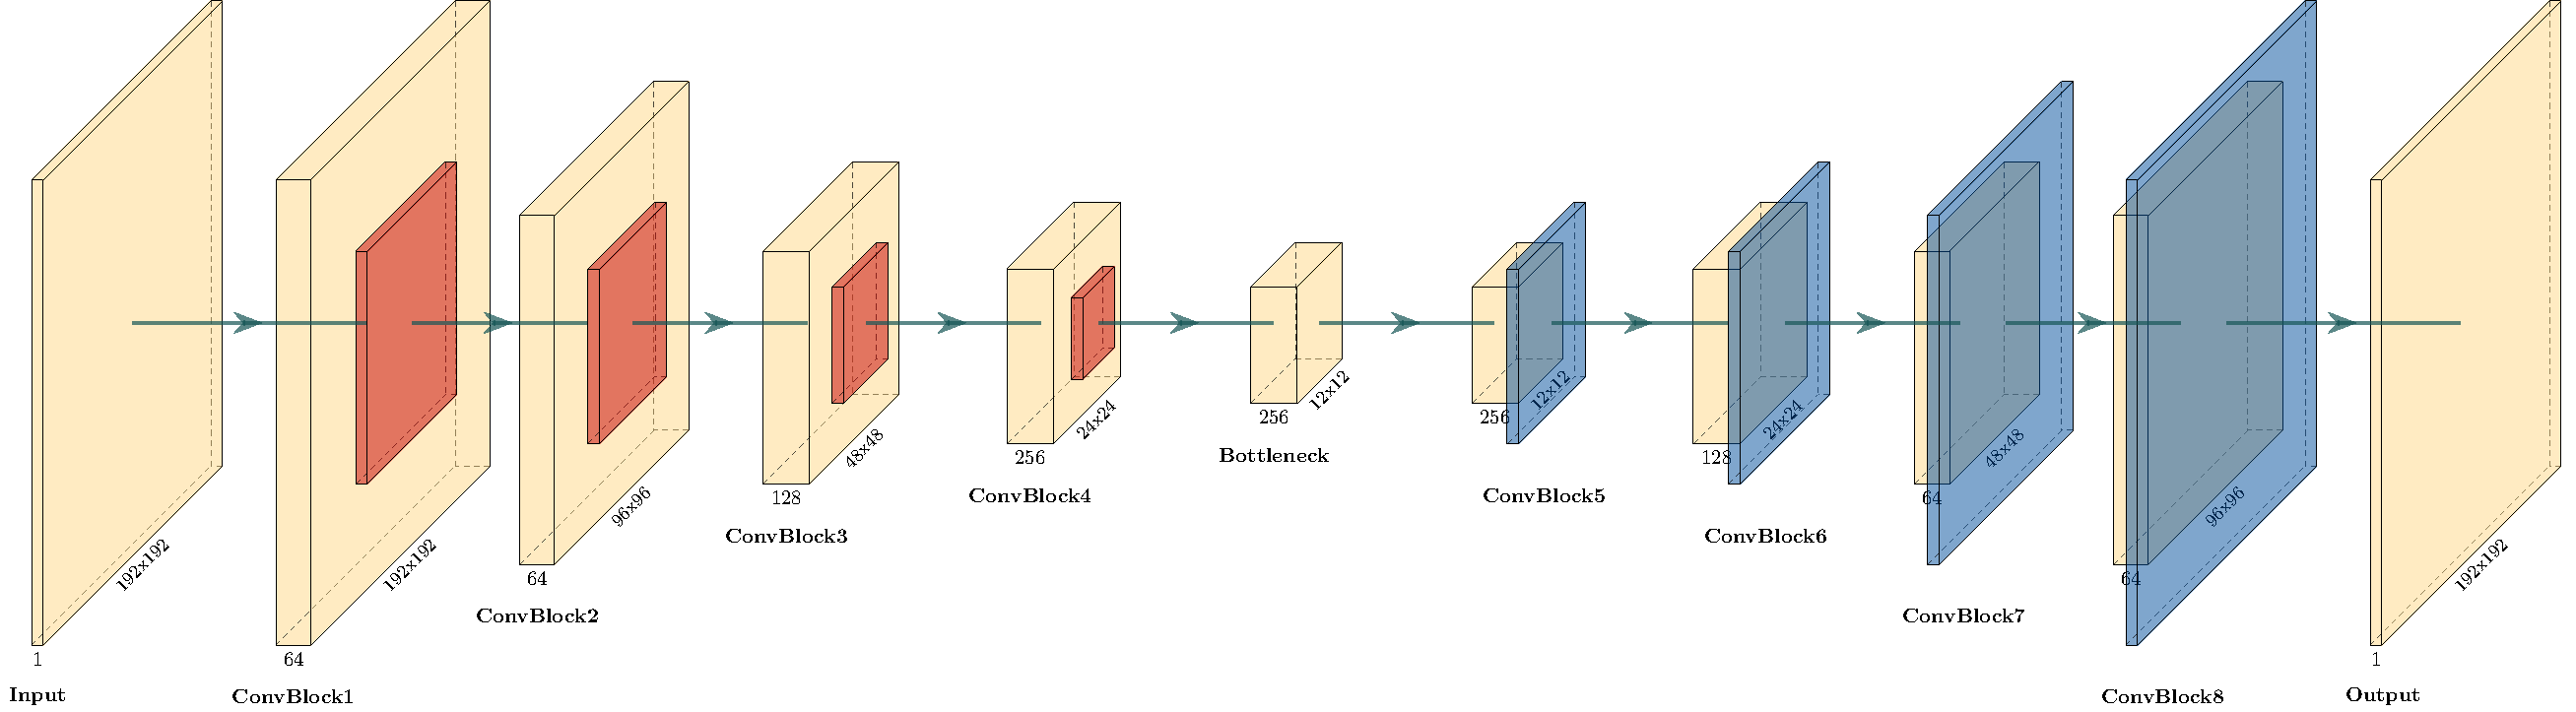
\includegraphics[width=\linewidth]{img/ch6/architectures/irfan.pdf}
    \caption{Modified convolutional encoder-decoder architecture inspired by Irfan et al. (2020) \cite{brito-loeza_novel_2020}. Each ConvBlock includes batch normalisation and ReLU activation, though these are not explicitly shown.}
    \label{fig:irfan2020-architecture}
\end{sidewaysfigure}

\subsection{U-Net}\label{subsec:unet}

The U-Net model, originally proposed by Ronneberger et al. in their seminal 2015 paper, \textit{U-Net: Convolutional Networks for Biomedical Image Segmentation} \cite{ronneberger_u-net_2015}, is an extremely successful and well-recognised benchmark encoder-decoder architecture. Originally developed for image segmentation tasks, U-Net is characterised by its symmetric design: an encoder path that progressively reduces spatial dimensions to capture contextual information, and a decoder path that reconstructs high-resolution outputs via up-sampling and skip connections. Its name comes from the U-shaped structure formed by the encoder, decoder, and the connecting skip connections.

Skip connections, first popularised by the ResNet architecture \cite{he_deep_2015}, are one of the key features in U-Net. They help gradients flow smoothly from the input to the output layers, making training more stable and addressing issues like the vanishing gradient problem \cite{adaloglou_intuitive_2020}. Additionally, these connections carry over spatial details lost during down-sampling in the encoder and combine them with features in the decoder. This ensures that the model reuses important details from earlier layers and maintains consistent dimensions, helping to merge fine-grained spatial information with the broader context captured by earlier layers.

In this study, the classification head of the original U-Net has been removed to focus exclusively on reconstruction tasks. The architectural details are summarised in Table \ref{tab:unet-model}, and the model is illustrated in Figure \ref{fig:unet-architecture}.

\begin{table}[htbp]
\centering
\caption{Layer-wise breakdown of the U-Net architecture. Convolutional layers are each followed by LeakyReLU activation (not explicitly shown).}
\label{tab:unet-model}
\renewcommand{\arraystretch}{1.25}
\begin{tabular}{lcccc}
\toprule
\textbf{Block} & \textbf{Layer Name} & \textbf{Filter Size} & \textbf{Output Shape} & \textbf{Connected to} \\ 
\midrule
\multirow{13}{*}{\textbf{Encoder}}
    & Input        & --           & $192 \times 192 \times 3$ & -- \\ 
    & Conv1        & $3 \times 3$ & $192 \times 192 \times 64$ & Input \\ 
    & Conv2        & $3 \times 3$ & $192 \times 192 \times 64$ & Conv1 \\ 
    & MaxPool1     & $2 \times 2$ & $96 \times 96 \times 64$  & Conv2 \\ 
    & Conv3        & $3 \times 3$ & $96 \times 96 \times 128$ & MaxPool1 \\ 
    & Conv4        & $3 \times 3$ & $96 \times 96 \times 128$ & Conv3 \\ 
    & MaxPool2     & $2 \times 2$ & $48 \times 48 \times 128$ & Conv4 \\ 
    & Conv5        & $3 \times 3$ & $48 \times 48 \times 256$ & MaxPool2 \\ 
    & Conv6        & $3 \times 3$ & $48 \times 48 \times 256$ & Conv5 \\ 
    & MaxPool3     & $2 \times 2$ & $24 \times 24 \times 256$ & Conv6 \\ 
    & Conv7        & $3 \times 3$ & $24 \times 24 \times 512$ & MaxPool3 \\ 
    & Conv8        & $3 \times 3$ & $24 \times 24 \times 512$ & Conv7 \\ 
    & MaxPool4     & $2 \times 2$ & $12 \times 12 \times 512$ & Conv8 \\ 
\midrule
\multirow{2}{*}{\textbf{Bottleneck}}
    & Conv9        & $3 \times 3$ & $12 \times 12 \times 1024$ & MaxPool4 \\ 
    & Conv10       & $3 \times 3$ & $12 \times 12 \times 1024$ & Conv9 \\ 
\midrule
\multirow{17}{*}{\textbf{Decoder}}
    & UpSample1    & $2 \times 2$ & $24 \times 24 \times 1024$ & Conv10 \\ 
    & Concatenate1 & --           & $24 \times 24 \times 1536$ & UpSample1, Conv8 \\ 
    & Conv11       & $3 \times 3$ & $24 \times 24 \times 512$  & Concatenate1 \\ 
    & Conv12       & $3 \times 3$ & $24 \times 24 \times 512$  & Conv11 \\ 
    & UpSample2    & $2 \times 2$ & $48 \times 48 \times 512$  & Conv12 \\ 
    & Concatenate2 & --           & $48 \times 48 \times 768$  & UpSample2, Conv6 \\ 
    & Conv13       & $3 \times 3$ & $48 \times 48 \times 256$  & Concatenate2 \\ 
    & Conv14       & $3 \times 3$ & $48 \times 48 \times 256$  & Conv13 \\ 
    & UpSample3    & $2 \times 2$ & $96 \times 96 \times 256$  & Conv14 \\ 
    & Concatenate3 & --           & $96 \times 96 \times 384$  & UpSample3, Conv4 \\ 
    & Conv15       & $3 \times 3$ & $96 \times 96 \times 128$  & Concatenate3 \\ 
    & Conv16       & $3 \times 3$ & $96 \times 96 \times 128$  & Conv15 \\ 
    & UpSample4    & $2 \times 2$ & $192 \times 192 \times 128$ & Conv16 \\ 
    & Concatenate4 & --           & $192 \times 192 \times 192$ & UpSample4, Conv2 \\ 
    & Conv17       & $3 \times 3$ & $192 \times 192 \times 64$  & Concatenate4 \\ 
    & Conv18       & $1 \times 1$ & $192 \times 192 \times 64$  & Conv17 \\ 
    & Output       & $1 \times 1$ & $192 \times 192 \times 3$   & Conv18 \\ 
\bottomrule
\end{tabular}
\end{table}

\begin{sidewaysfigure}
    \centering
    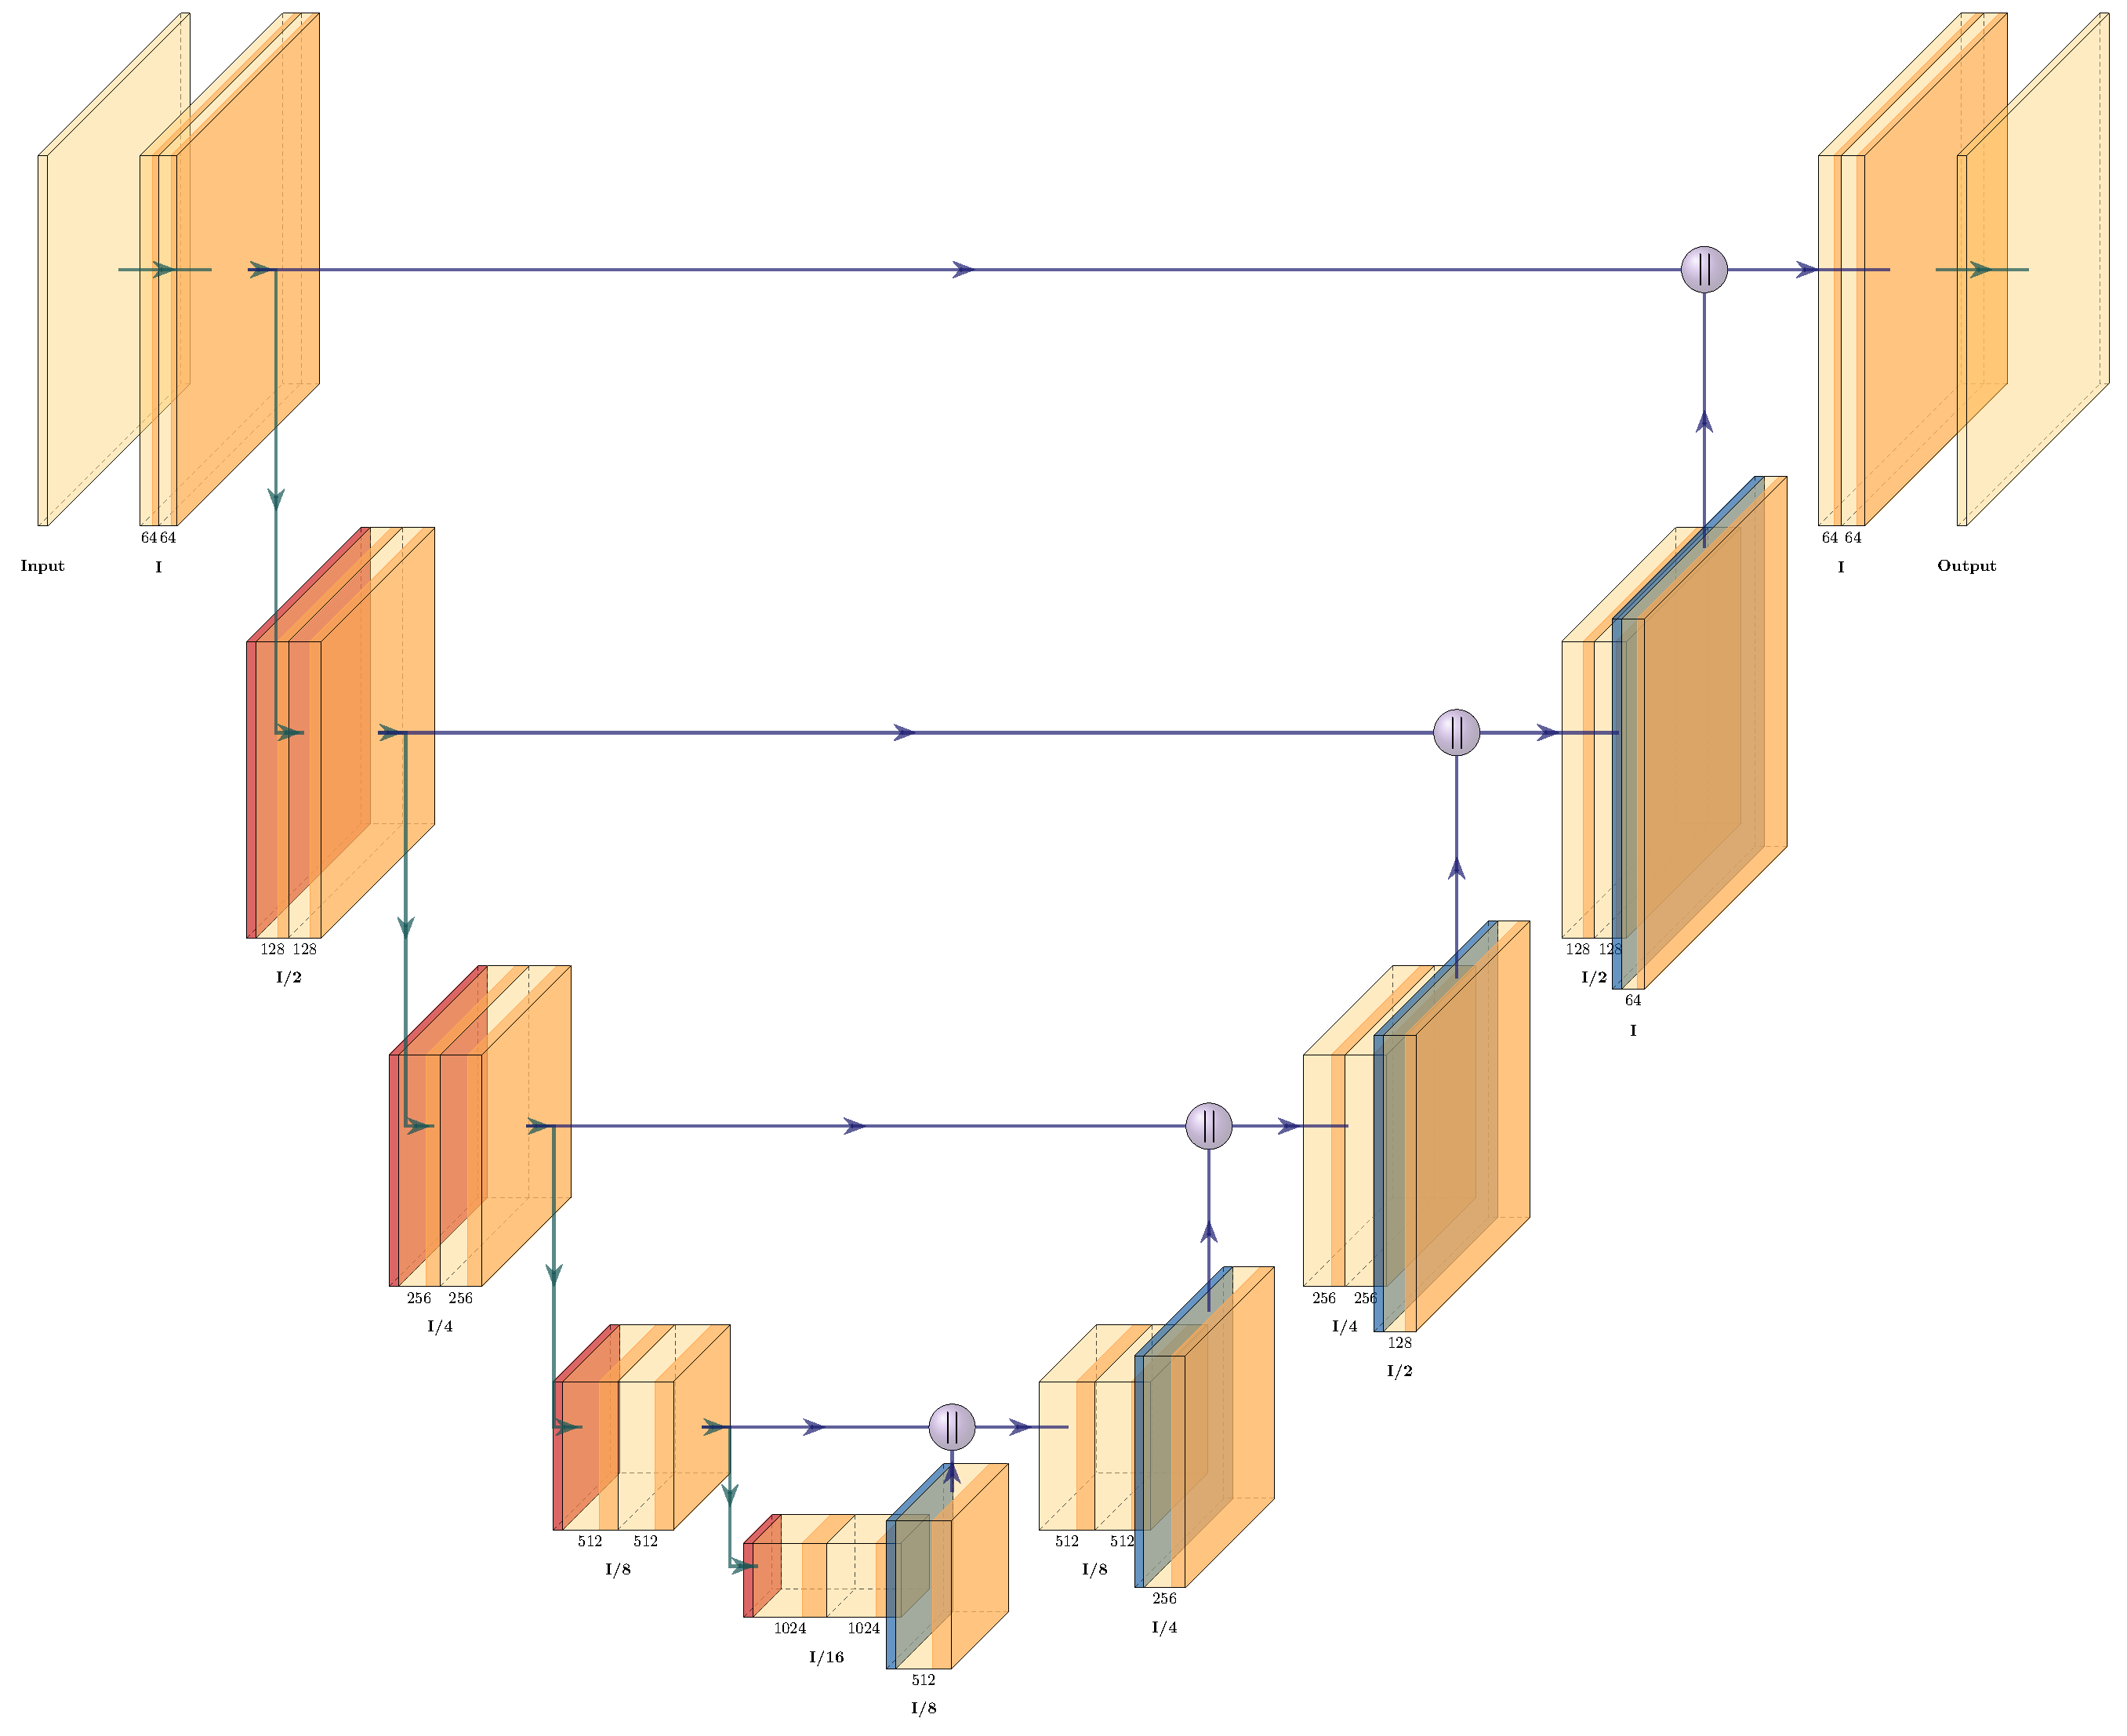
\includegraphics[width=0.80\paperwidth, keepaspectratio]{img/ch6/architectures/unet.pdf}
    \caption{Illustration of the U-Net architecture \cite{ronneberger_u-net_2015} with its classification layer removed, resulting in a fully symmetric encoder-decoder structure.}
    \label{fig:unet-architecture}
\end{sidewaysfigure}

\section{Overview of benchmark datasets used}\label{sec:denoising-datasets}

To evaluate the performance of our denoising methods, we used two well-established natural image datasets as benchmarks: ImageNet and the Berkeley Segmentation Dataset (BSD). 

\subsection{ImageNet}

ImageNet \cite{deng_imagenet_2009} is a landmark dataset widely used for training and benchmarking computer vision models. It consists of over 15 million high-resolution images categorised into approximately 22,000 classes, collected from web sources such as Flickr. Since 2010, the dataset has served as the foundation for the annual ImageNet Large Scale Visual Recognition Challenge (ILSVRC) \cite{russakovsky_imagenet_2015}, which has been pivotal in driving breakthroughs in deep learning architectures, such as AlexNet \cite{krizhevsky_imagenet_2012}, ResNet \cite{he_deep_2015}, and Vision Transformers \cite{dosovitskiy_image_2020}.

For this chapter, we utilised the ILSVRC 2012 dataset, a widely used subset of ImageNet consisting of 1.2 million training images, 50,000 validation images, and 150,000 test images, evenly distributed across 1,000 object categories. Due to computational constraints, we worked with a subset of the validation set, specifically the first 10,000 images. This reduced dataset provided a practical sample for our experiments.

\subsection{Berkeley Segmentation Dataset}

The Berkeley Segmentation Dataset \cite{martin_database_2001} is a widely used benchmark dataset in computer vision, particularly for tasks involving image segmentation and denoising. Unlike datasets designed for model training, BSD is primarily used for evaluating the performance of algorithms across metrics such as \acrshort{psnr}. The dataset consists of 300 natural images, divided into 200 training images and 100 testing images. The images are sourced from everyday scenes, including landscapes, objects, and urban settings, and have been manually annotated to facilitate segmentation tasks. For this chapter, we used the test set of 100 images for the evaluation of our methods on natural images.

% \subsection{Synthetic spectrograms}

% To bridge the gap between natural image datasets like ImageNet and the noisy spectrograms of the DeepShip dataset, we generated a synthetic spectrogram dataset. These synthetic spectrograms were created from simple signals, such as sine waves, with added Gaussian noise. This allowed us to explore denoising techniques in a controlled environment, providing a smooth transition from natural image experiments to real-world underwater acoustic data.

% The synthetic dataset was constructed on the fly using Python's SciPy library. First, sine waves with randomly selected frequencies were generated, mimicking basic tonal patterns. Gaussian noise with a random standard deviation, sampled from a predefined range, was then added to simulate the complexity of real-world underwater noise. This method of adding Gaussian noise with a random variance is well-established in scientific literature as a way to train models for denoising tasks \cite{lehtinen_noise2noise_2018}. Each noisy signal was then transformed into a power spectrogram to to ensure compatibility with our DeepShip inputs (Section \ref{sec:inputs}).

% \section{Experiment 1: Basic unsupervised denoising}

% \subsection{Methodology}

% What would happen if we just fed the same noisy image as both input and output of these models? Will they be able to denoise it?

% In our DeepShip generator, we have a toggle for \texttt{X\_only}. When this is toggled, the generator will simply return the same spectrogram twice, once for input to the model and once for the target.

% We split the dataset into 3
% %train_df, val_df, test_df = data.generate_kth_fold(fold_dfs, test_idx=1, val_idx=0)

% \subsection{Results}

% \begin{table}[htbp] 
% \centering 
% \caption{Denoising performance of Irfan and U-Net models on DeepShip spectrograms for Experiment 2.} 
% \label{tab:denoising-exp-2-results} 
%     \begin{tabular}{lccc} 
%     \toprule 
%     \textbf{Model} & \textbf{Epochs} & \textbf{Loss} & \textbf{\acrshort{psnr} (dB)}\\ \midrule 
%     Irfan & 50 & $8.30 \times 10^{-3}$ & 20.91 \\
%     U-Net & 15 & $2.73 \times 10^{-6}$ & 55.92 \\
%     \bottomrule
%     \end{tabular} 
% \end{table}

% \begin{figure}[p]
%     \centering
%     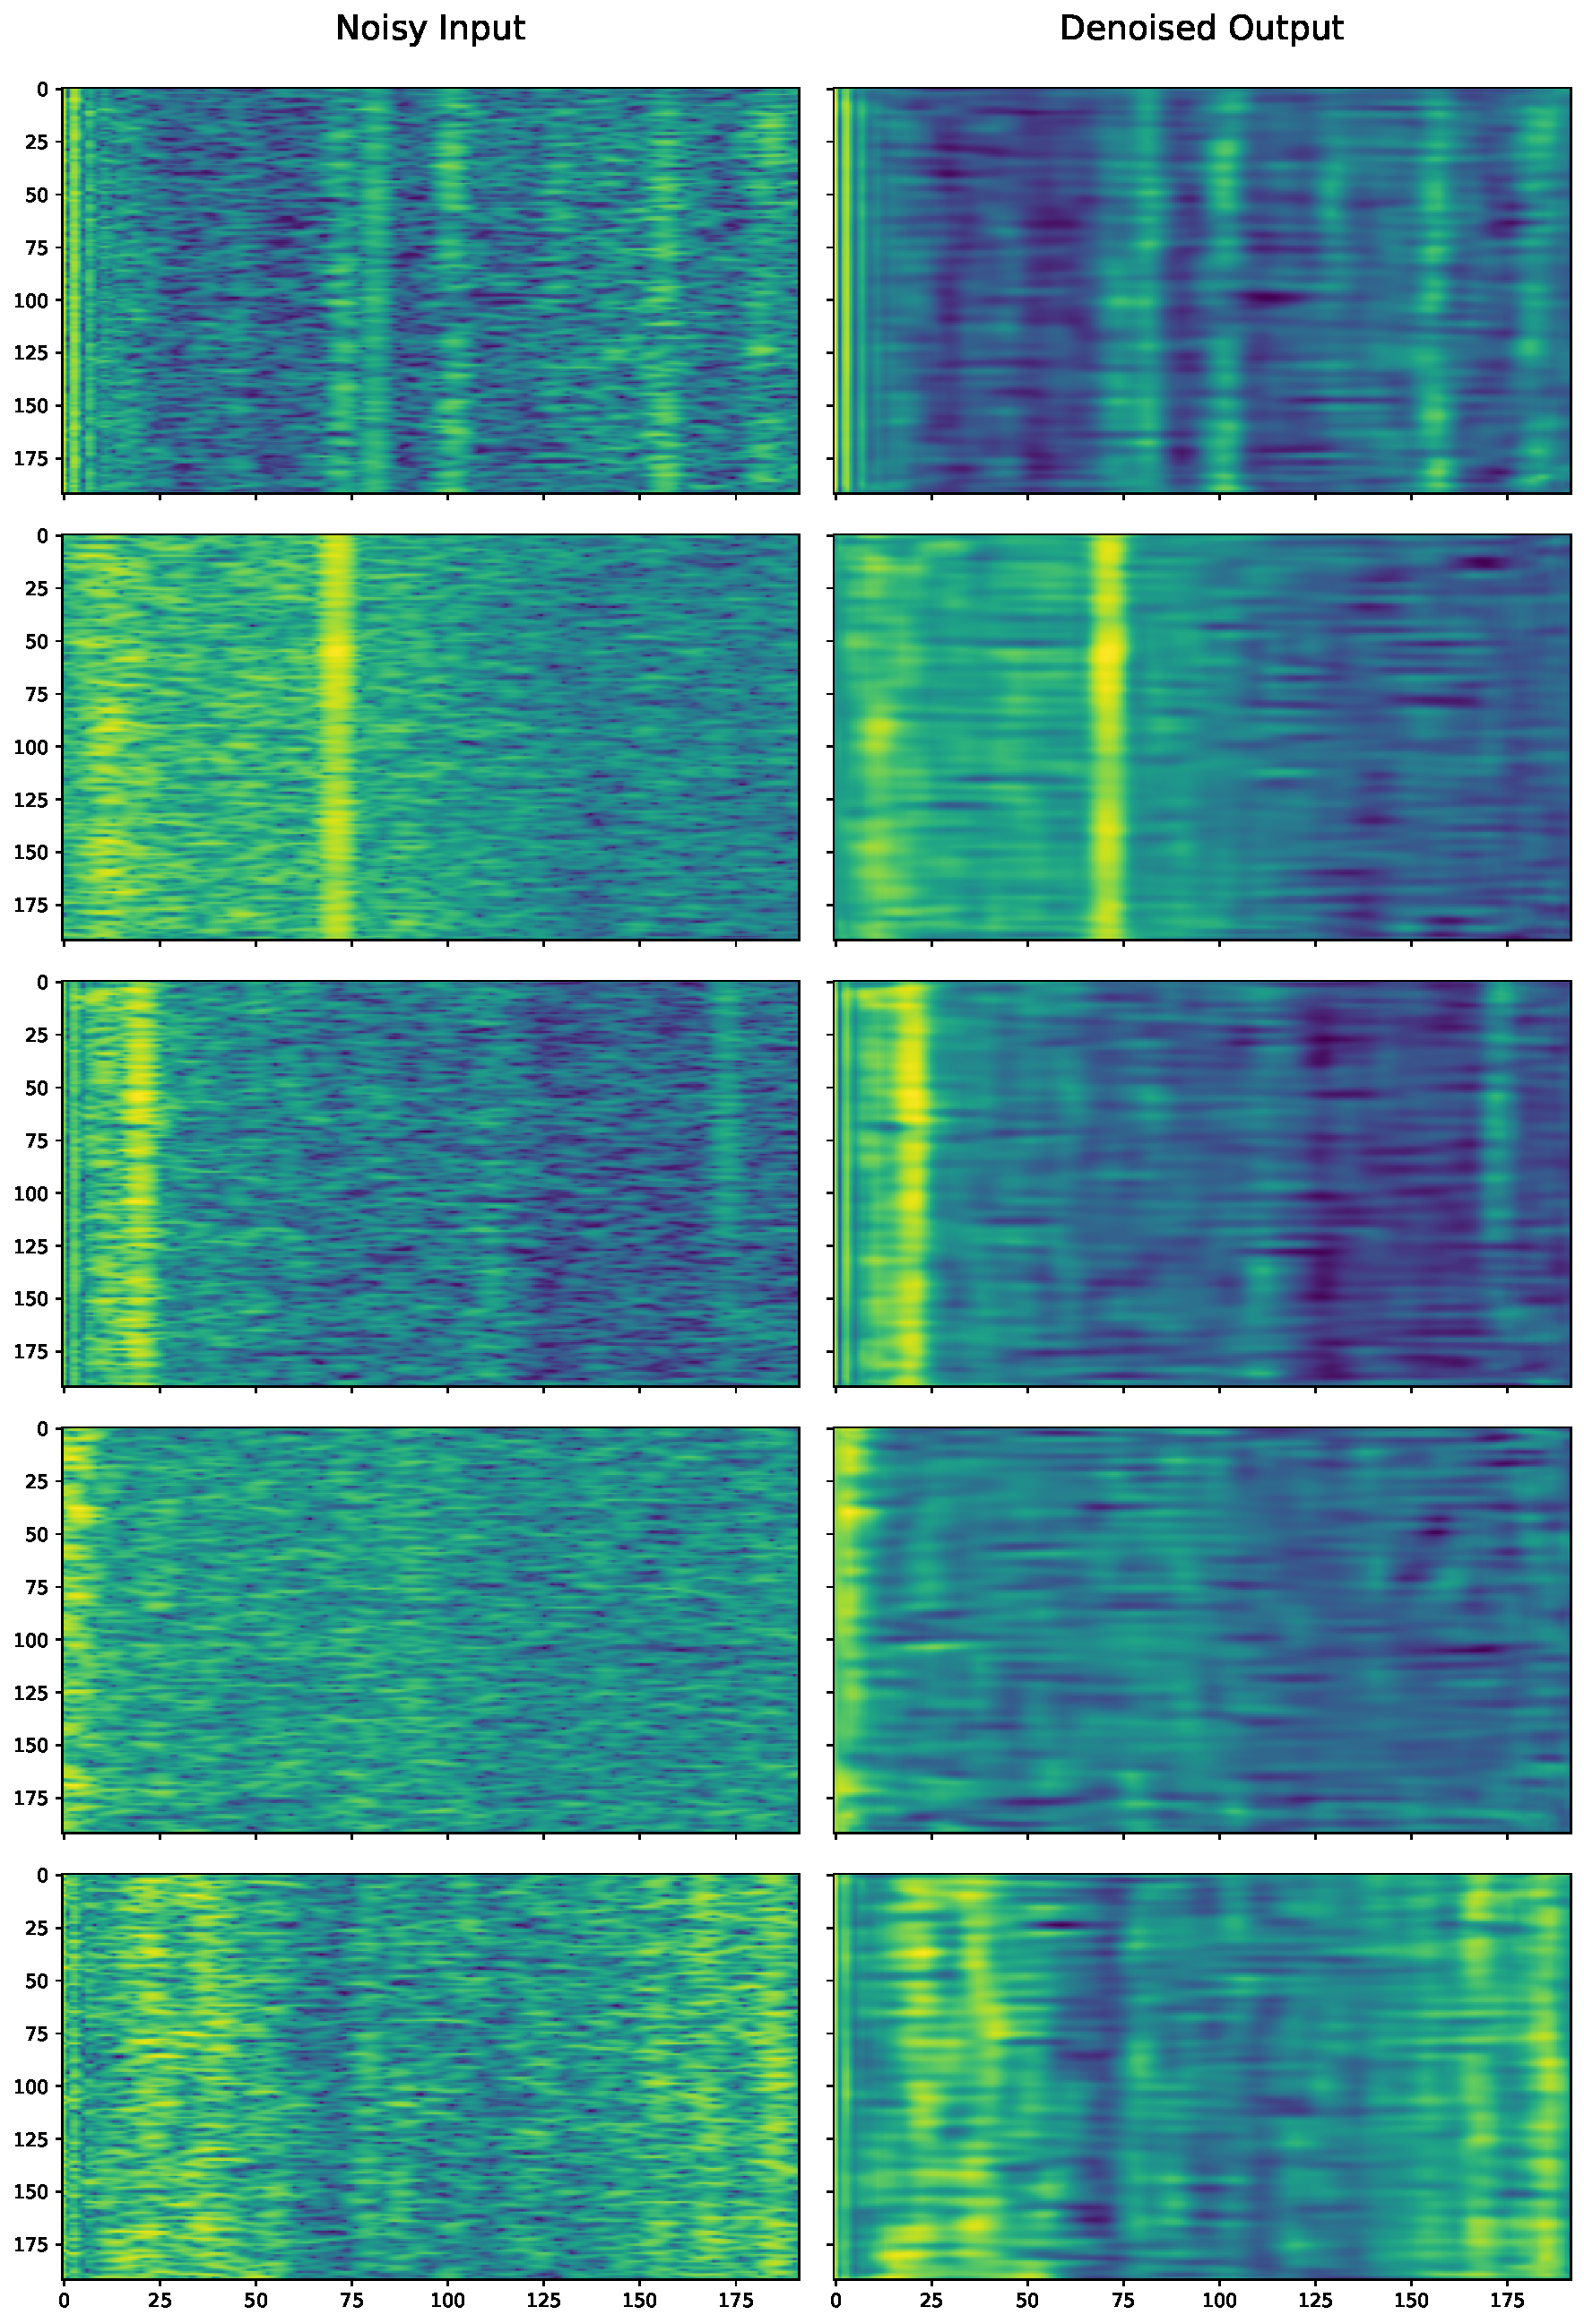
\includegraphics[width=0.95\textwidth]{img/ch6/in_eq_out/irfan/combined_spectrograms.pdf}
%     \caption{Sample results of Experiment 2 with the Irfan model. The left column shows the original input, while the right column shows the denoised output. There is minimal visual difference between the two.}
%     % \label{fig:enter-label}
% \end{figure}

% \begin{figure}[p]
%     \centering
%     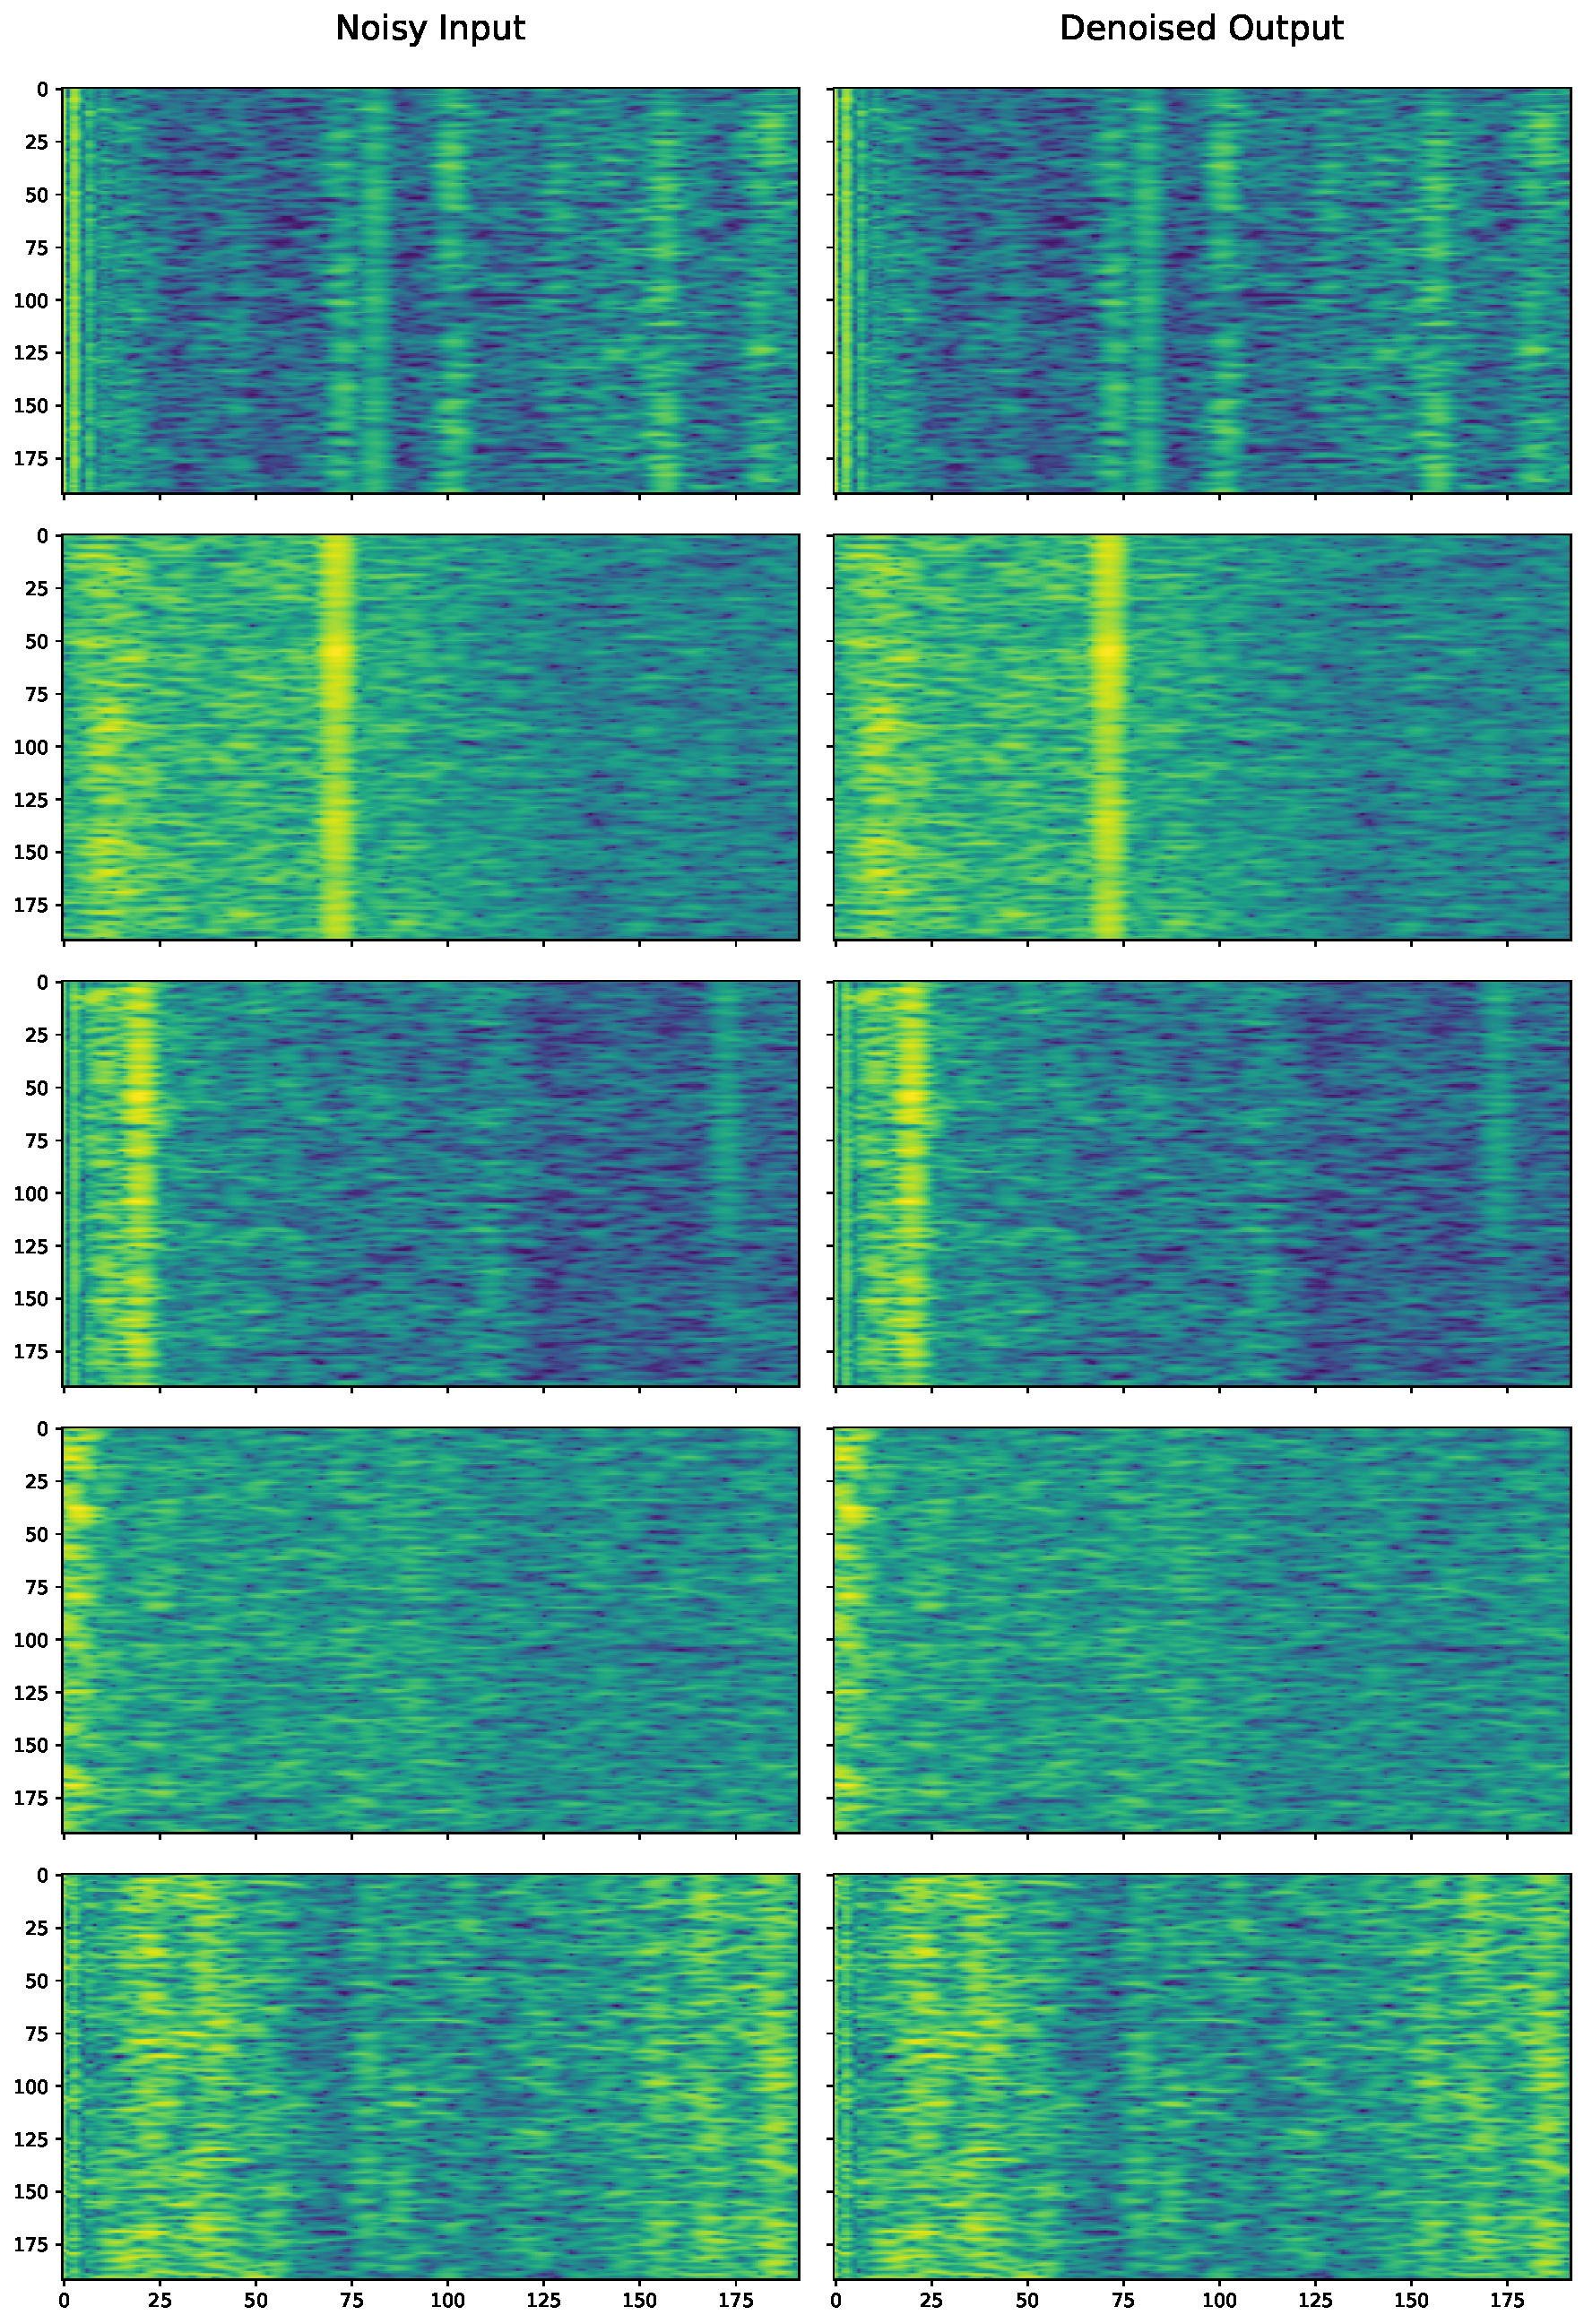
\includegraphics[width=0.95\textwidth]{img/ch6/in_eq_out/unet/combined_spectrograms.pdf}
%     \caption{Sample results of Experiment 2 with the U-Net model. The left column shows the original input, while the right column shows the denoised output. There is minimal visual difference between the two.}
%     % \label{fig:enter-label}
% \end{figure}

% \subsection{Discussion}

% \lipsum[1-5]

% \begin{figure}[htbp]
%     \centering
%     \begin{subfigure}{\textwidth}
%         \centering
%         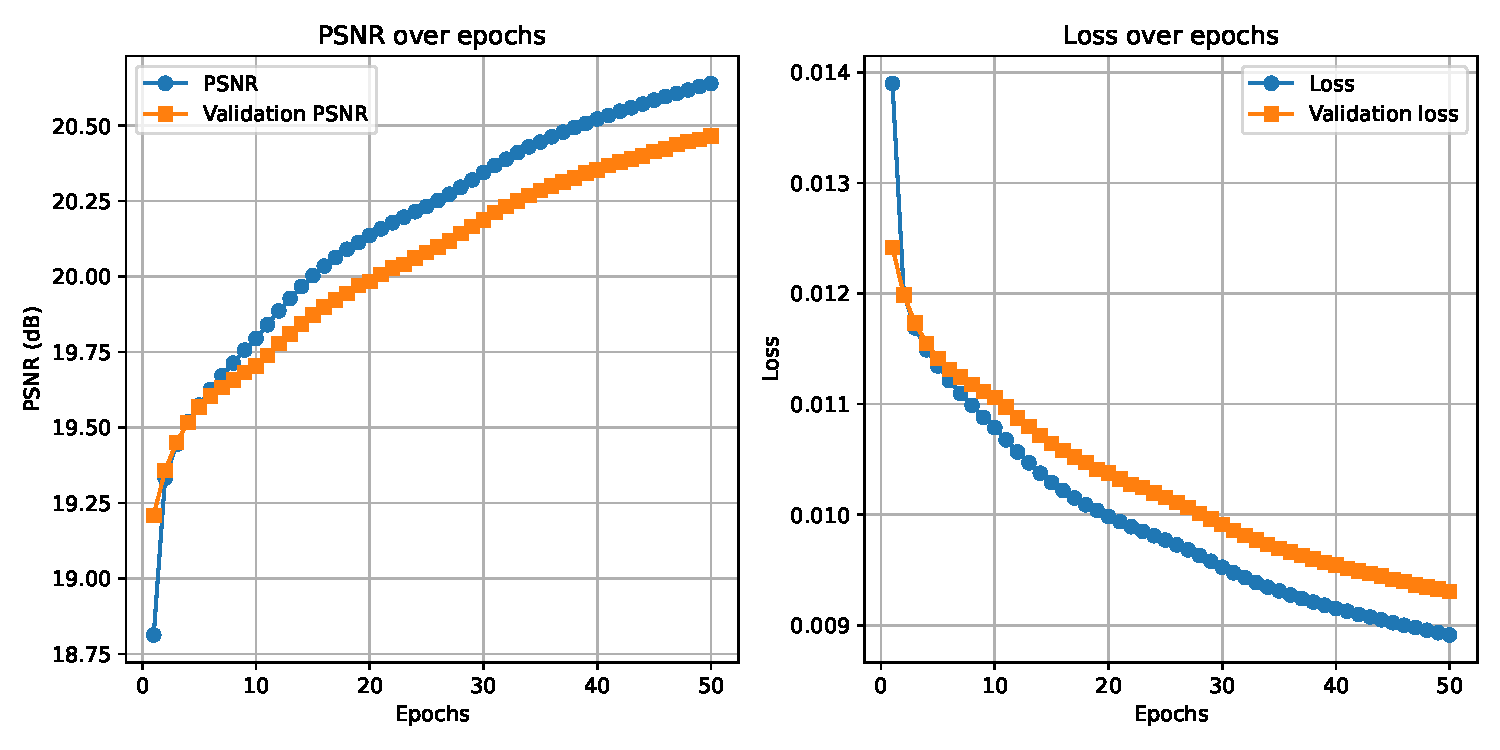
\includegraphics[width=\textwidth]{img/ch6/in_eq_out/irfan/psnr_loss_curves.pdf}
%         \caption{\acrshort{psnr} and loss curves for the Irfan model, trained over 50 epochs.}
%         \label{fig:denoising-exp2-curves-irfan}
%     \end{subfigure}
    
%     \vspace{0.5cm}
    
%     \begin{subfigure}{\textwidth}
%         \centering
%         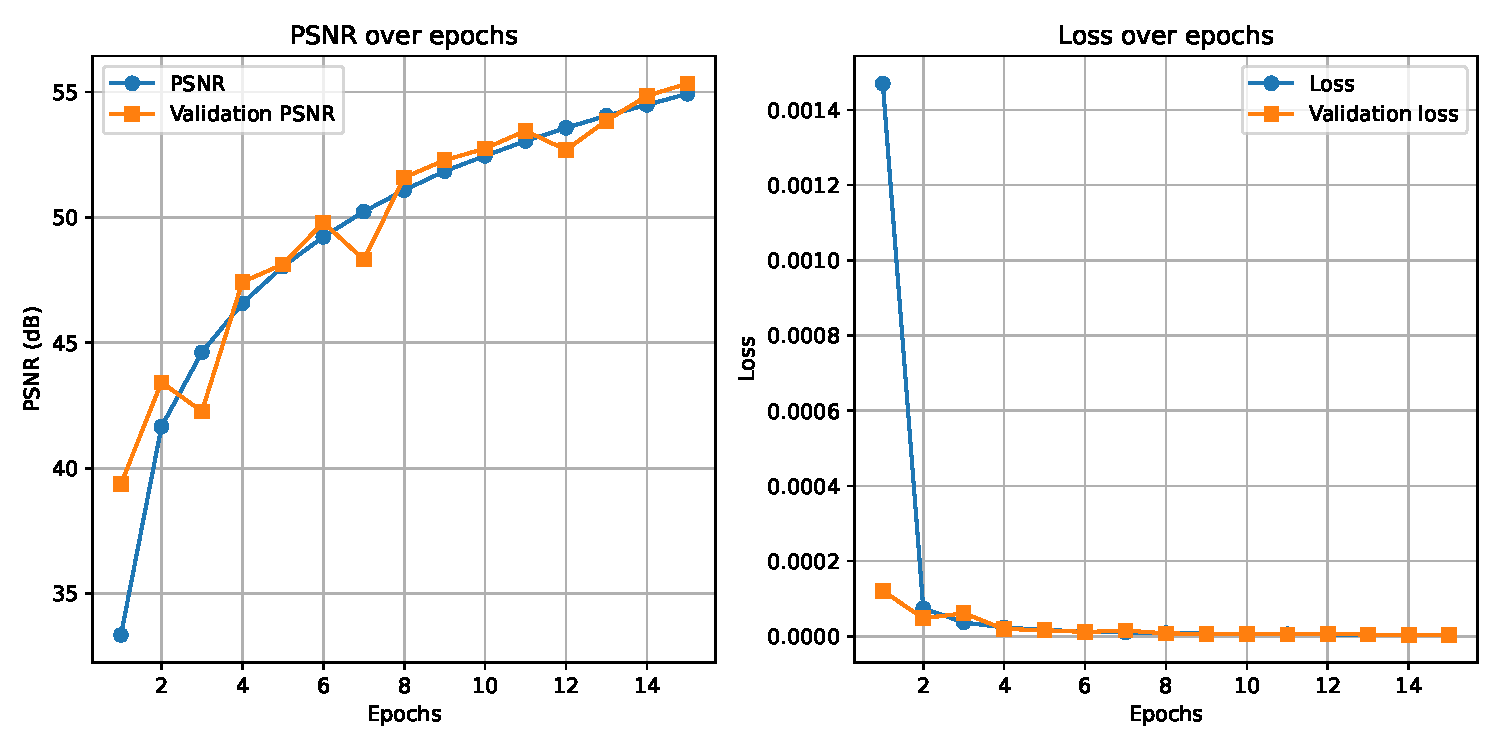
\includegraphics[width=\textwidth]{img/ch6/in_eq_out/unet/psnr_loss_curves.pdf}
%         \caption{\acrshort{psnr} and loss curves for the U-Net model, trained over 15 epochs due to time constraints.}
%         \label{fig:denoising-exp2-curves-unet}
%     \end{subfigure}
%     \caption{\acrshort{psnr} and loss curves for the (a) Irfan and (b) U-Net models for Experiment 1.}
%     \label{fig:denoising-exp2-curves}
% \end{figure}

% \subsubsection{Future work}

% TALK ABOUT U-NETPRO HERE.

% \subsection{Conclusion}

% \lipsum[1-2]

% \newpage
\section{Experiment 1: Unsupervised denoising with Noise2Noise}

The Noise2Noise framework offers an innovative approach to denoising, bypassing the need for clean labels by leveraging pairs of noisy samples with uncorrelated noise. As outlined in Section \ref{sec:denoising-techniques}, this methodology has demonstrated remarkable success in domains where these assumptions hold true. The objective of this experiment is twofold: first, to validate the Noise2Noise approach by recreating its performance on natural images; and second, to investigate its applicability to underwater acoustic spectrograms, a domain where these assumptions are challenging to approximate.

This experiment is structured into two parts. In the first part, we replicate the Noise2Noise framework using natural images, employing two models, Irfan and U-Net, to benchmark their performance. This serves as a baseline validation of the methodology, and verification of the results originally presented in the Noise2Noise paper. In the second part, we extend the framework to underwater acoustic spectrograms, testing its performance under the specific assumptions and constraints of this domain. This section examines whether Noise2Noise can effectively handle the complexities of underwater acoustics, including dynamic noise conditions and the absence of clean paired data.

Ultimately, this experiment seeks to provide insights into the strengths and limitations of Noise2Noise, offering a foundation for its future application to underwater acoustic signal processing. We conclude by reflecting on the challenges encountered and proposing directions for further research.

\subsection{Part I: Recreating the original paper}\label{subsec:recreating-n2n}

This section aims to validate the performance of the Noise2Noise methodology on natural images by recreating the original paper as authentically as possible using our two chosen architectures: U-Net and the Irfan model. By replicating the Gaussian noise experiments from the original Noise2Noise paper \cite{lehtinen_noise2noise_2018}, we demonstrate the viability of the approach before applying it to underwater acoustic spectrograms.

\subsubsection{Methodology}

Our methodology closely follows the original Noise2Noise framework, with some modifications to accommodate our experimental setup and computational constraints. Note that the original paper compares their technique traditional supervised denoising; thus, we also implement a traditional denoiser using both Irfan and U-Net for comparison.

\paragraph{Training Noise2Noise}
In line with the original paper, we began by taking clean images from the ImageNet validation set and extracting a random square patch of $192 \times 192$ pixels from the image. Each patch was then processed to generate two distinct noisy versions by applying Gaussian noise with a standard deviation randomly sampled from the range $[0, 50]$, as specified in the original paper. This process created noisy image pairs $(x, x')$, with one noisy image $x$ serving as the model input, while the other $x'$ acting as the target label. This setup ensured compliance with the Noise2Noise assumption that paired noisy inputs share the same underlying distribution.

\paragraph{Training a supervised denoiser}
For comparison, we also trained a traditional supervised denoiser on the ImageNet validation set. In this case, a random $192 \times 192$ pixel patch was extracted from each image, but instead of applying two different noise distributions, only one was applied. This process created noisy-clean pairs $(y, x)$.

\paragraph{}
At the end of each epoch, the performance of all models was evaluated using a validation set consisting of the BSD300 training images. The validation generator produced pairs $(y, x)$, allowing us to compute the \acrshort{psnr} by directly comparing the denoised output $\hat{y}$ with the ground truth, $y$.

Finally, after training, each model was evaluated on the BSD test set. As before, a random $192 \times 192$ pixel crop was extracted from each test image, and Gaussian noise with a random standard deviation was applied. The noisy patch was fed into the model for evaluation, with the denoised outputs compared to the clean originals. The \acrshort{psnr} values were recorded to assess the effectiveness of Noise2Noise on natural images and to provide a direct performance comparison between the U-Net and Irfan architectures.

\subsubsection{Implementation and training setup}

We implemented the training and validation pipelines in Python using TensorFlow. The implementation was designed with flexibility in mind, offering options to toggle 0-1 normalised inputs, convert images to greyscale or retain RGB channels, and switch between multiple noise distributions if required. For 0-1 normalised inputs, the standard deviation of the Gaussian noise was scaled by a factor of 255 to match the scaled pixel intensity range.

Our training setup aimed to follow the original paper as faithfully as possible: the minibatch size was set to 4 for training and evaluation, training was conducted using the ADAM optimiser \cite{kingma_adam_2014}, with $\beta_1 = 0.9$, $\beta_2 = 0.99$, and $\epsilon = 10^{-8}$, \acrfull{mse} was used as the loss function, and \acrshort{psnr} served as the primary evaluation metric. 

For the U-Net model, weights were initialised using He initialisation \cite{he_delving_2015} for stable convergence. No batch normalization, dropout, or other regularisation techniques were used, following the original methodology. Finally, LeakyReLU with $\alpha = 0.1$ \cite{maas_rectifier_2013} was employed after each convolutional layer except the final one.

Our complete implementation of Noise2Noise can be found on the project GitHub repository.

\subsubsection{Adjustments to original settings}

While our goal was to faithfully recreate the Noise2Noise paper, several adjustments were made to align with our specific experimental setup and resource constraints:
\begin{itemize}
    \item The original paper explored multiple including Poisson, and Bernoulli distributions. However, as our aim here was primarily verification of the method, we decided to focus exclusively on Gaussian noise for simplicity and computational efficiency.
    \item In the original paper, the authors conducted some of their initial experiments using an architecture called RED30 \cite{mao_image_2016} but quickly switched to U-Net as it was ``roughly 10x faster'' while still giving ``similar results'' \cite[3]{ronneberger_u-net_2015}. Here, we simply used the U-Net and Irfan architectures for our experiment.
    \item Due to computational limitations, we used a subset of 10,000 images from the ImageNet validation set instead of the full 50,000 images. 
    \item For similar reasons, we also limited training for the U-Net model to 50 epochs compared to the original 150 epochs \cite[Fig 1.]{lehtinen_noise2noise_2018}. 
    \item The image patches extracted from the images were $192 \times 192$ pixels rather than the $256 \times 256$ stated in the original implementation, in order to ensure consistency with the resolution of DeepShip spectrograms.
    \item Our experiments were conducted on grayscale images (1 channel), reflecting the single-channel nature of spectrograms, whereas the original paper worked with RGB images (3 channels).
    \item The paper used $[-0.5, 0.5]$ normalisation, while we chose to use $[0, 1]$ normalisation as it is a more standard technique including when dealing with spectrograms.
    \item The original paper used a learning rate of $10^{-3}$, but preliminary experiments showed suboptimal results with this setting. We adjusted this to $10^{-5}$ for more stable training.
    \item Unlike the original, which did not specify a validation set, we introduced a validation step using BSD300's training set which contains 200 images. Nevertheless, evaluation was still conducted on BSD300's testing set of 100 images, as the original paper called for.
\end{itemize}

\subsubsection{Results}

The results of our recreation of the Noise2Noise paper closely align with those obtained by the original authors. The Irfan model achieved a \acrshort{psnr} of 22.15 dB on the BSD testing set, while the U-Net model, a deeper and more sophisticated architecture, achieved 29.59 dB. This result is slightly below the 31.06 dB obtained by Lehtinen et al. \cite[3]{lehtinen_noise2noise_2018}, who trained their model for 100 more epochs than we did. A visualisation of the Noise2Noise model outputs is presented in Figure \ref{fig:n2n-recreation}. Additionally, Figure \ref{fig:n2n-vs-supervised} compares the outputs from supervised and unsupervised models.

\begin{table}[htbp] 
\centering 
\caption{Performance of the Irfan and U-Net models on the BSD testing set for our recreation of the Noise2Noise paper.} 
\label{tab:n2n-imagenet-results} 
    \begin{tabular}{lcccc} 
    \toprule 
    \textbf{Strategy} & \textbf{Model} & \textbf{Loss} & \textbf{\acrshort{psnr} (dB)} \\ \midrule 
    \multirow{2}{*}{Supervised} & Irfan & 0.0094 & 21.48 \\
    & U-Net & 0.0017 & 29.78 \\
    \addlinespace
    \multirow{2}{*}{Noise2Noise} & Irfan & 0.0080 & 22.15\\
    & U-Net & 00.18 & 29.59\\ \bottomrule
    \end{tabular} 
\end{table}

\begin{figure}[p]
    \centering
    \begin{subfigure}{\textwidth}
        \centering
        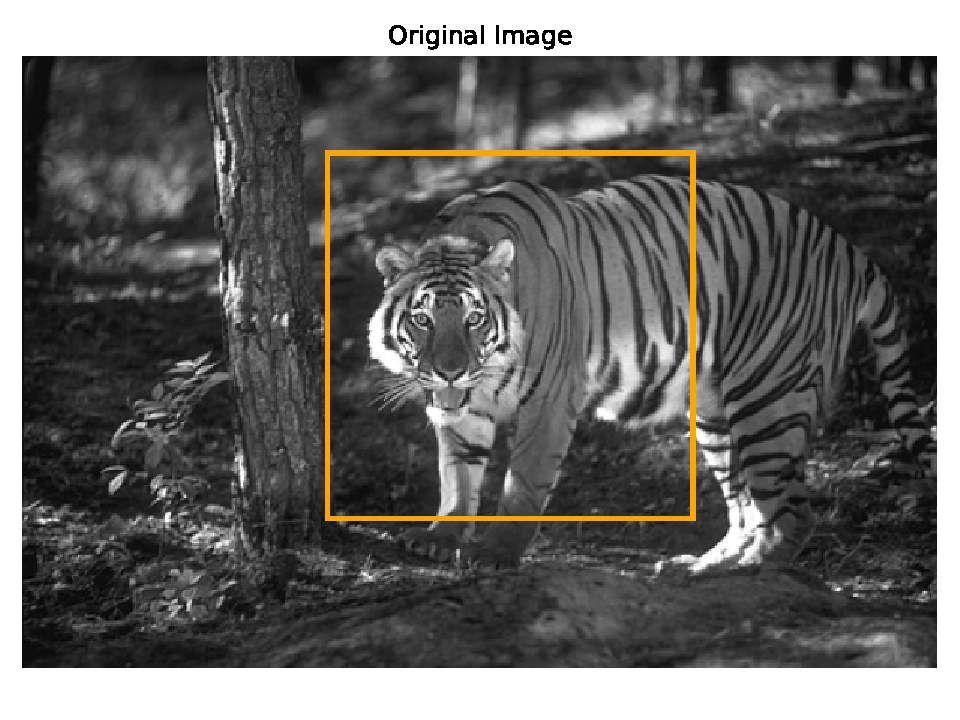
\includegraphics[trim={0 0.35cm 0 0.85cm},clip,width=0.49\linewidth]{img/ch6/n2n_imagenet/ground_truth_1.pdf}
        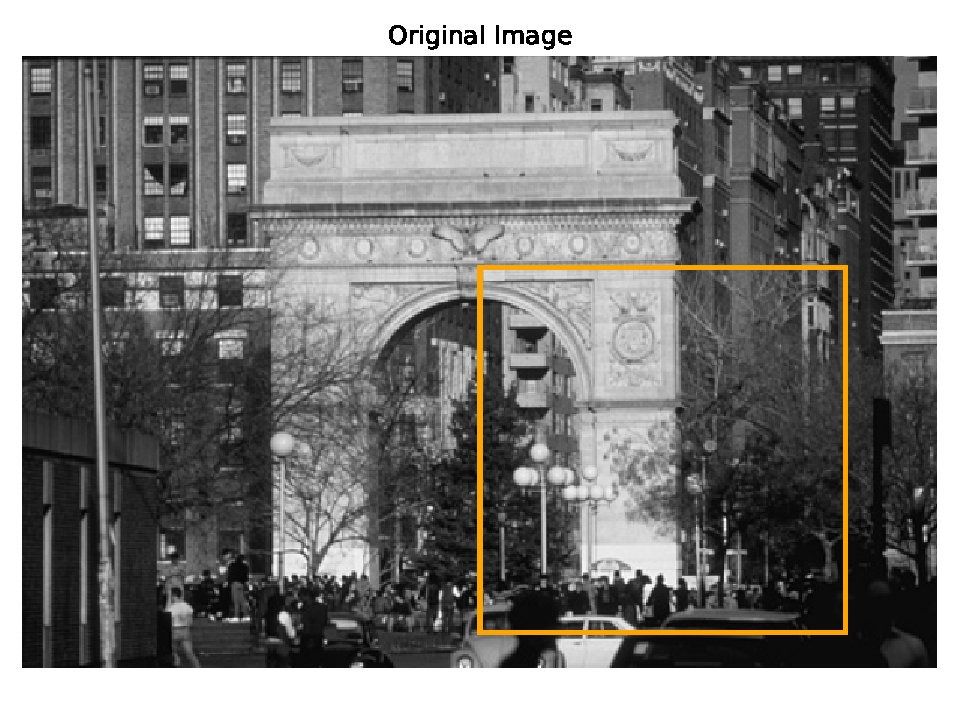
\includegraphics[trim={0 0.35cm 0 0.85cm},clip,width=0.49\linewidth]{img/ch6/n2n_imagenet/ground_truth_2.pdf}
        \caption{Raw ground truth images used for visual evaluation with $192 \times 192$ patches highlighted.}
        \label{fig:n2n-recreation-ground-truth}
    \end{subfigure}

    \vspace{0.5cm}

    \begin{subfigure}{\textwidth}
        \centering
        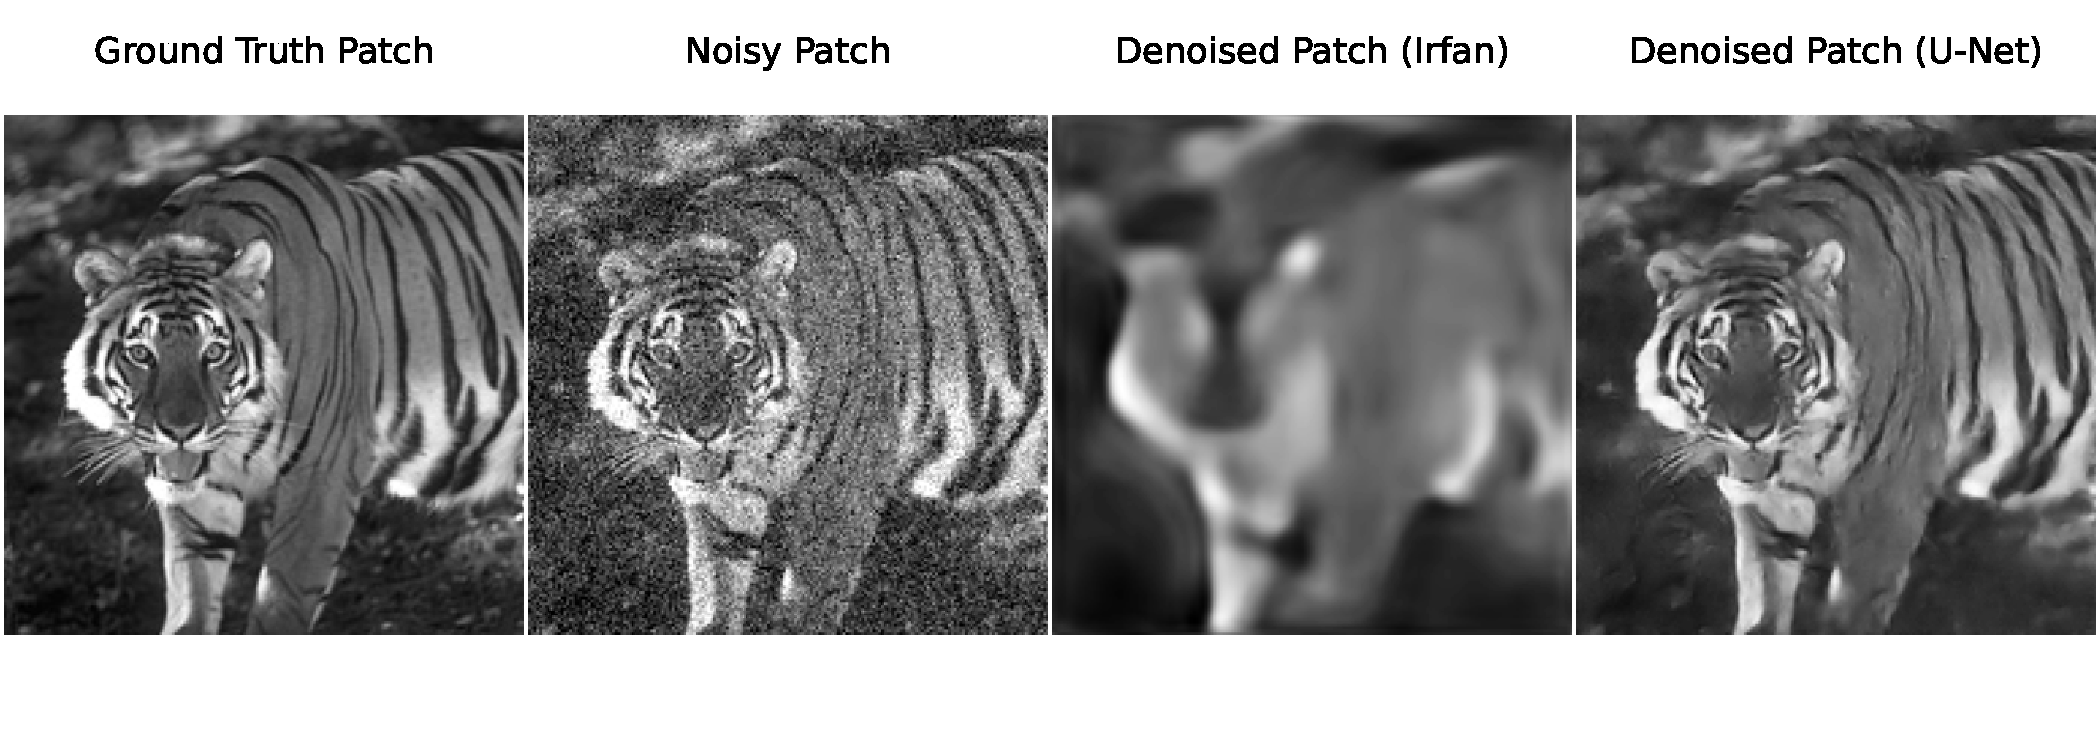
\includegraphics[trim={0 1cm 0 0},clip,width=\textwidth]{img/ch6/n2n_imagenet/irfan_vs_unet_1.pdf}
        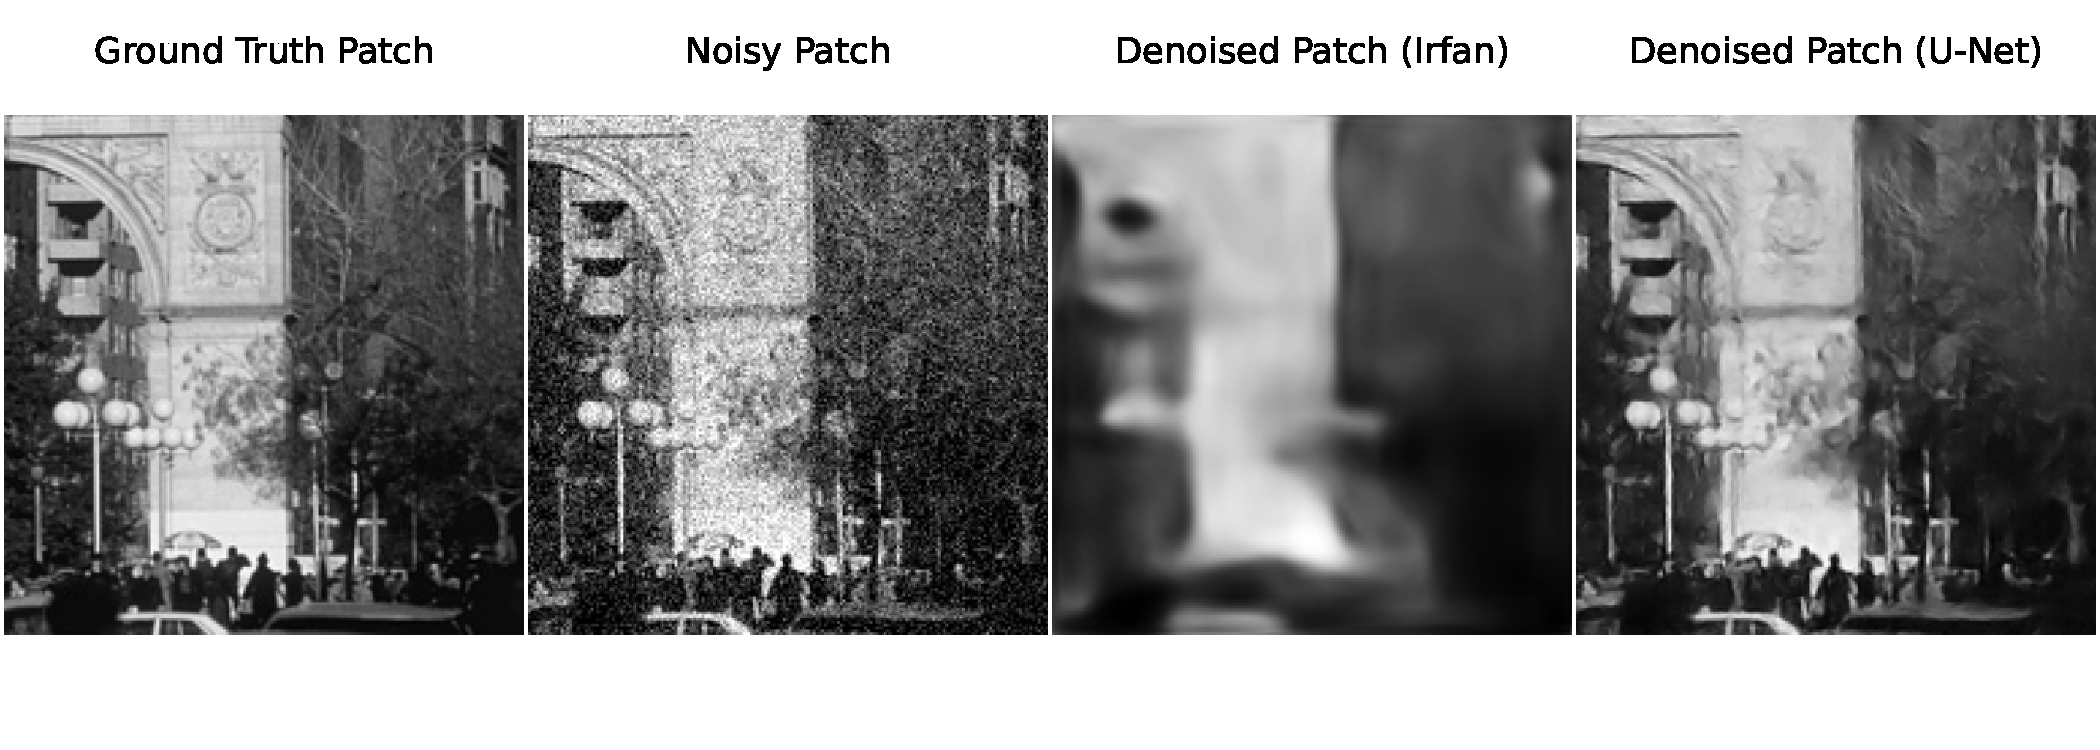
\includegraphics[trim={0 1cm 0 2cm},clip,width=\textwidth]{img/ch6/n2n_imagenet/irfan_vs_unet_2.pdf}
        \caption{Comparison of ground truth patches, noisy patches, the Irfan model output, and the U-Net model output.}
        \label{fig:n2n-recreation-comparison}
    \end{subfigure}
    \caption{Visual comparison of ground truth images, noisy patches, and denoised model outputs for our Noise2Noise recreation.}
    \label{fig:n2n-recreation}
\end{figure}

\begin{figure}[p]
    \centering
    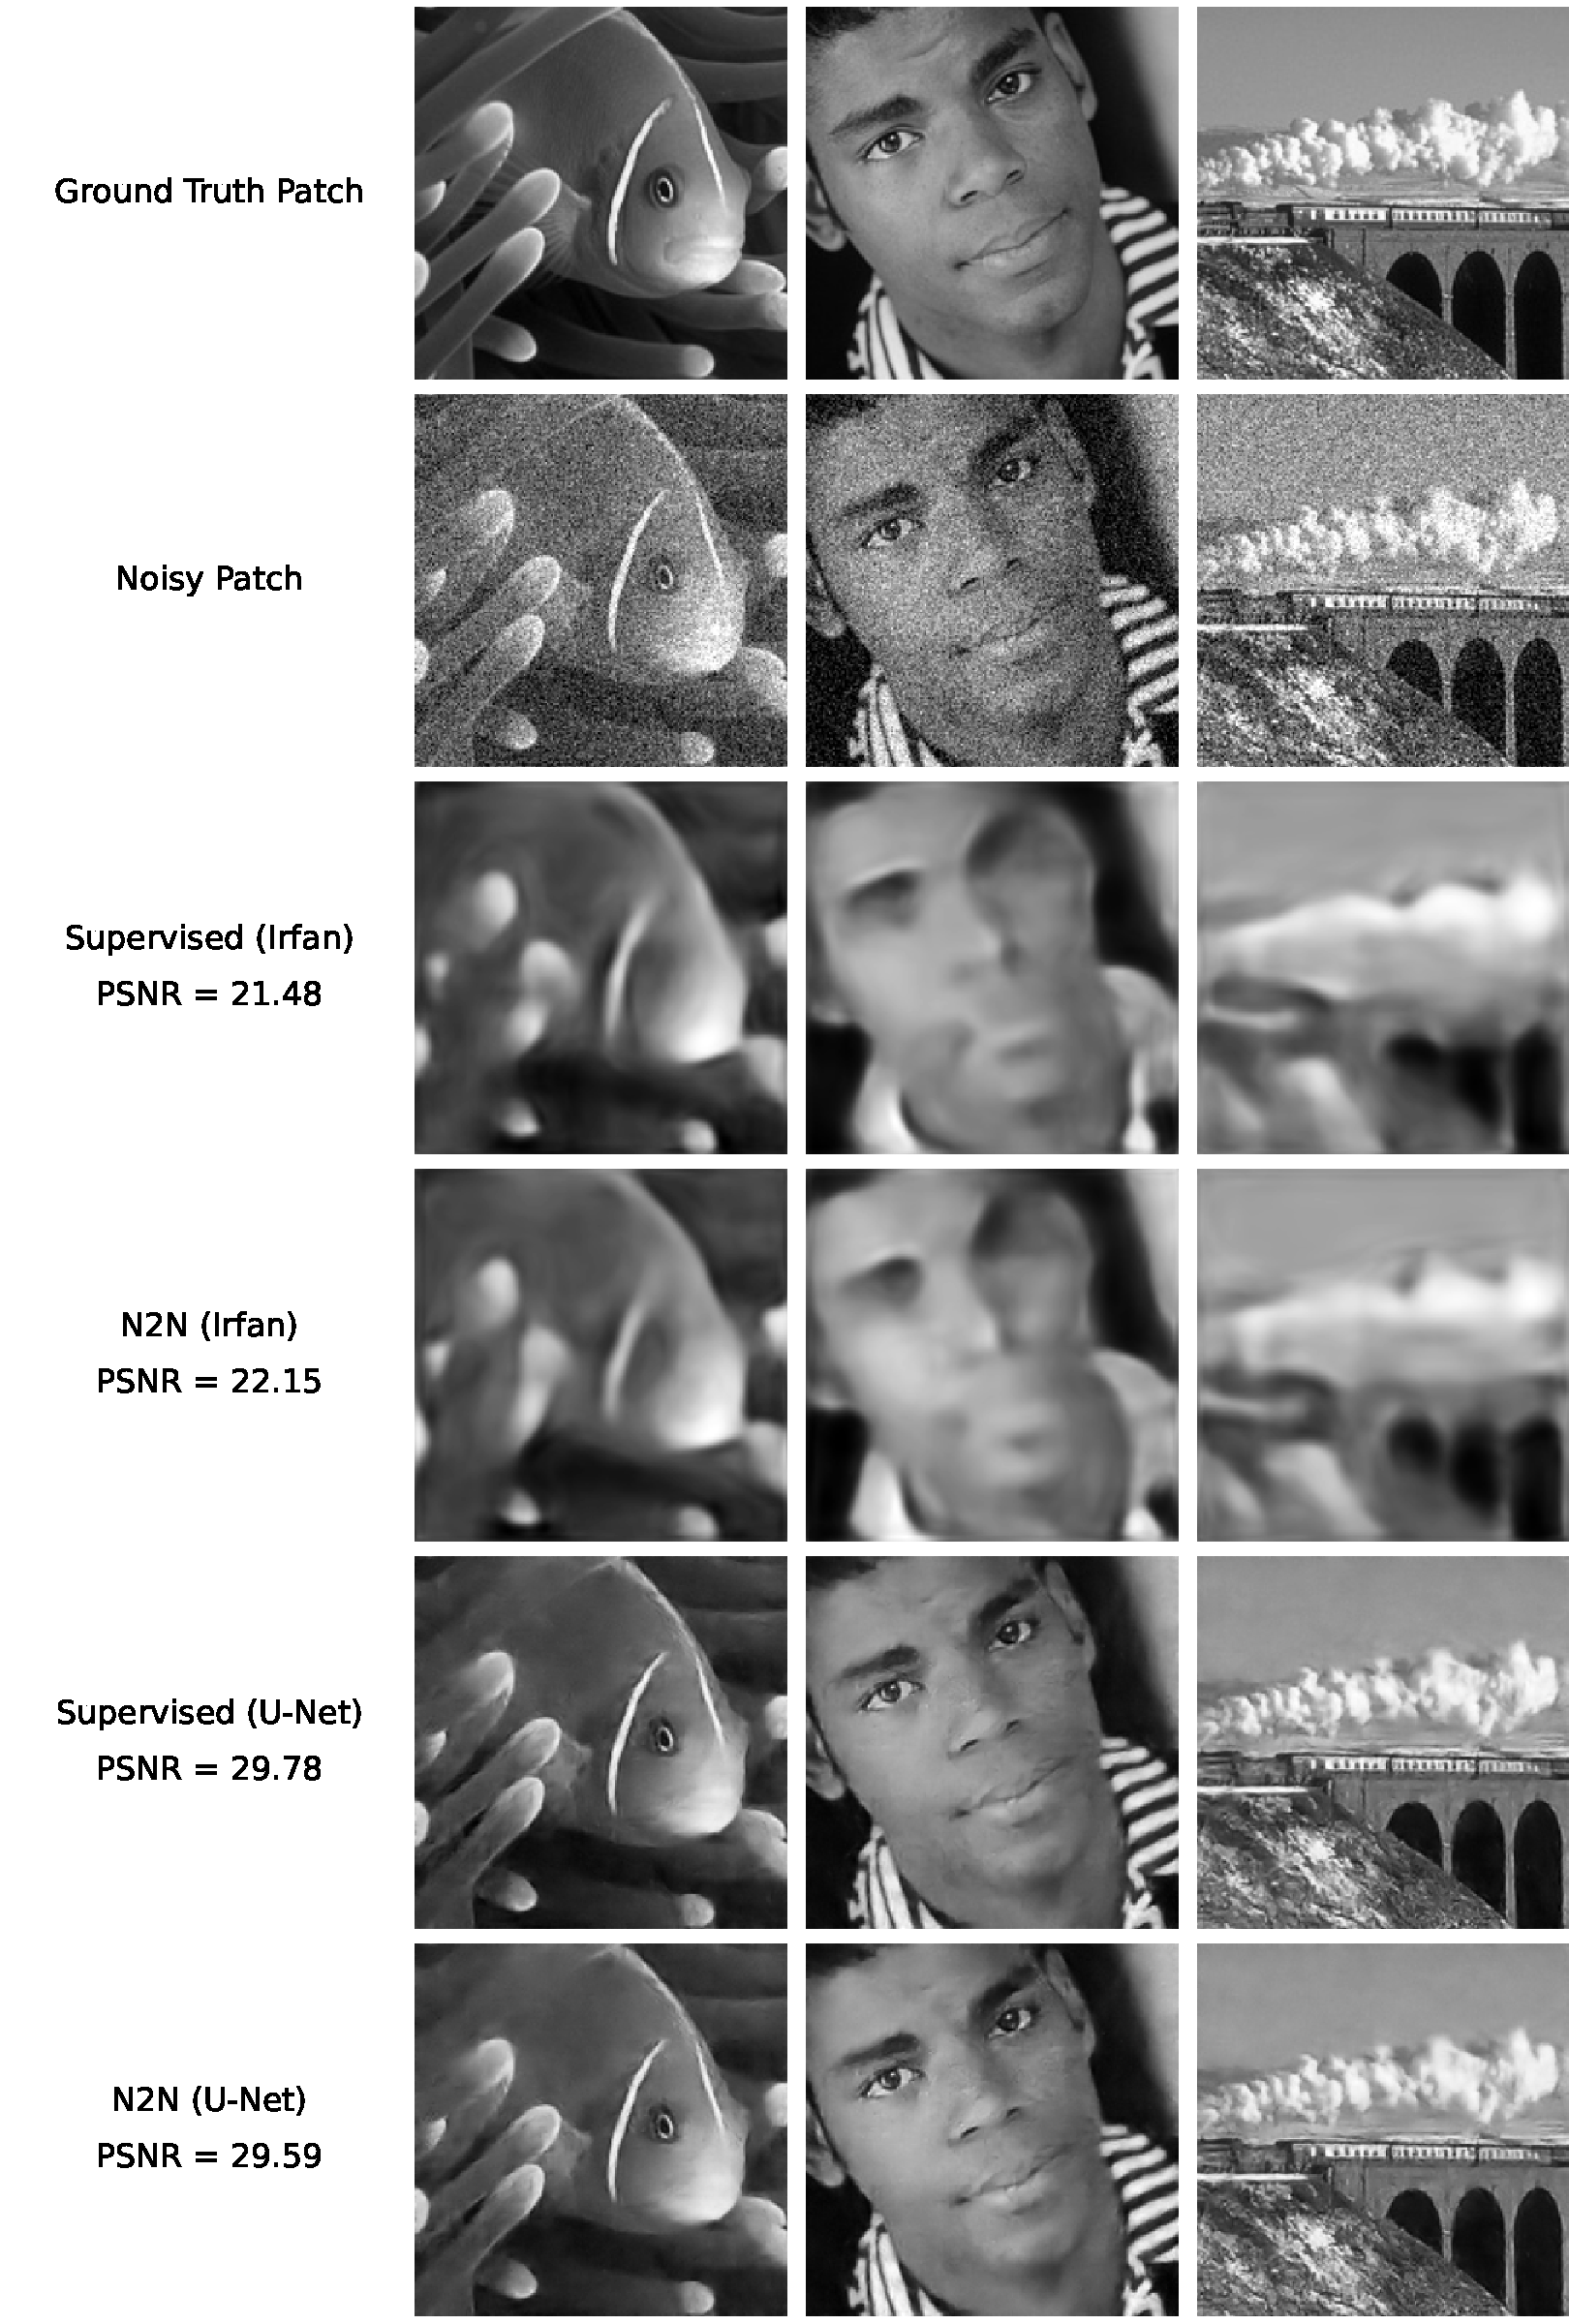
\includegraphics[width=0.9\textwidth]{img/ch6/n2n_imagenet/denoising_comparison_2.pdf}
    \caption{Comparison of supervised and Noise2Noise denoising methods applied to both the Irfan and U-Net models.}
    \label{fig:n2n-vs-supervised}
\end{figure}

\subsubsection{Discussion}

The results of this experiment validate the effectiveness of the Noise2Noise methodology, with the unsupervised model achieving performance nearly identical to that of the supervised model in terms of \acrshort{psnr}. This outcome is consistent with the findings of the original Noise2Noise paper \cite{lehtinen_noise2noise_2018}. Additionally, the outputs from both the supervised and unsupervised models (Figure \ref{fig:n2n-vs-supervised}) appear nearly identical, reinforcing the idea that the Noise2Noise approach performs on par with supervised learning techniques in terms of visual quality. This highlights the groundbreaking nature of the Noise2Noise methodology, where noise reduction can be achieved without the need for clean target images, a challenge that has faced traditional supervised denoising techniques for decades.

Interestingly, the Irfan model trained with Noise2Noise slightly outperformed its supervised counterpart in \acrshort{psnr} and loss values. This minor discrepancy may stem from the inherent regularisation effect of Noise2Noise training, which uses noisy targets and potentially mitigates overfitting to specific clean patterns. However, the difference is small enough to conclude that both models perform similarly in practice, as further supported by the nearly identical visual outputs.

A comparison between the Irfan and U-Net architectures reveals more pronounced differences, particularly in their ability to capture fine details. U-Net consistently outperformed Irfan in reconstructing intricate features, such as the tiger’s stripes (test/108005), the fine facial details of a man (test/302008), and the complex outlines and shading in the Washington Square Arch image (test/148089). In contrast, the Irfan model often produced blurry and less detailed outputs, failing to preserve critical image structures. Even in cases where both models succeeded at broader reconstructions, such as discerning the arches of the bridge in the steam train image (test/182053), U-Net demonstrated superior fidelity in capturing nuanced details like the shading of steam.

This performance discrepancy can be attributed to the architectural differences between Irfan and U-Net. Despite both Irfan and U-Net being convolutional encoder-decoder structures at heart, U-Net's success over Irfan is largely due to its skip connections, which allow the network to retain spatial information that would otherwise be lost during downsampling in the encoder. As discussed in Section \ref{subsec:unet}, these connections help merge both high-level and low-level features, enabling U-Net to effectively reconstruct both macro and micro details in the images. On the other hand, Irfan, a purely sequential model, lacks this feature and thus cannot effectively capture fine-grained spatial details, leading to poorer performance in reconstructing complex image structures. This architectural limitation underscores why U-Net is widely considered a state-of-the-art model for image reconstruction tasks.

Examining the training curves (Figures \ref{fig:supervised-denoising-curves} and \ref{fig:n2n-denoising-imagenet-curves}) further supports these findings. All models demonstrated stable convergence, with \acrshort{psnr} values plateauing around the 50th epoch. While training to the originally intended 150 epochs would have been ideal, the computational constraints of this experiment limited training to 50 epochs, with each model requiring over 24 hours to train on the available hardware. The supervised model's training and validation curves were closely aligned, indicating a well-fitted model with minimal overfitting. Conversely, the Noise2Noise model showed slightly lower training \acrshort{psnr} compared to validation \acrshort{psnr}, which is consistent with the methodology's reliance on noisy targets for training.

\begin{figure}[p]
    \centering
    \begin{subfigure}{\textwidth}
        \centering
        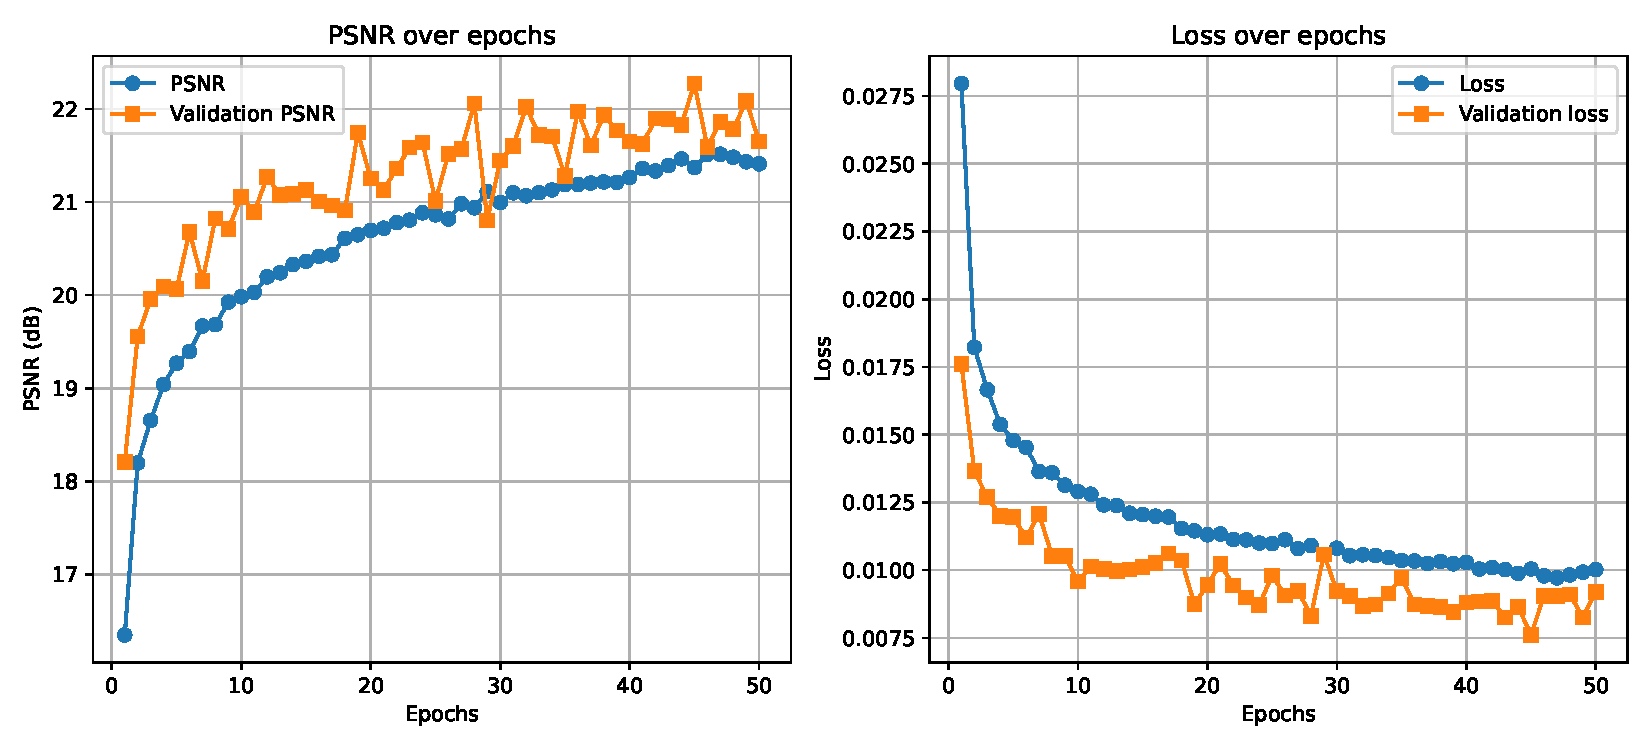
\includegraphics[width=\textwidth]{img/ch6/supervised/psnr_loss_irfan.pdf}
        \caption{\acrshort{psnr} and loss curves for Irfan (supervised denoising).}
    \end{subfigure}
    
    \vspace{1cm}
    
    \begin{subfigure}{\textwidth}
        \centering
        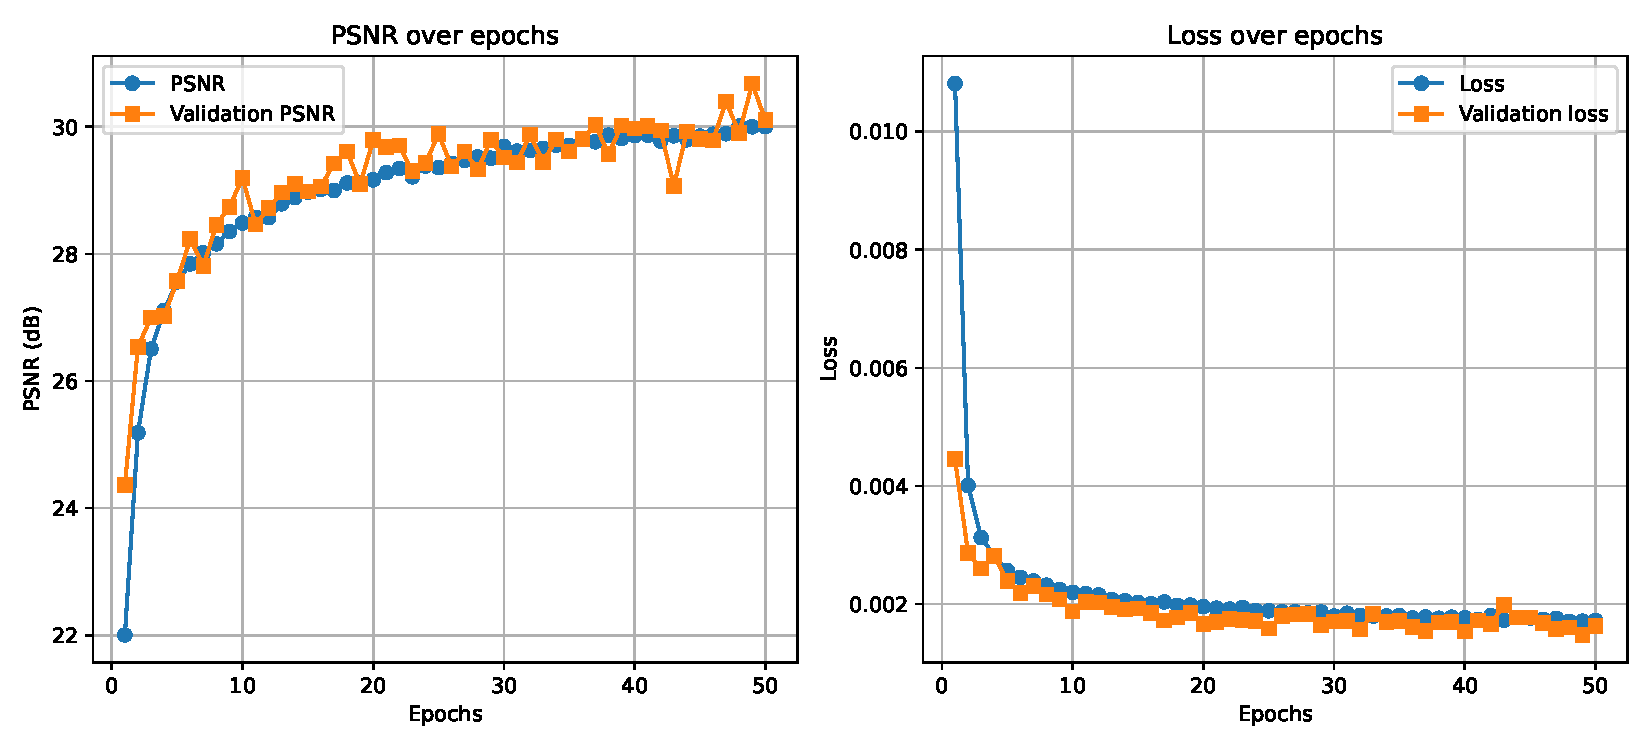
\includegraphics[width=\textwidth]{img/ch6/supervised/psnr_loss_unet.pdf}
        \caption{\acrshort{psnr} and loss curves for U-Net (supervised denoising).}
    \end{subfigure}
    \caption{\acrshort{psnr} and loss curves for the supervised denoising models trained on (a) Irfan and (b) U-Net.}
    \label{fig:supervised-denoising-curves}
\end{figure}
\begin{figure}[p]
    \centering
    \begin{subfigure}{\textwidth}
        \centering
        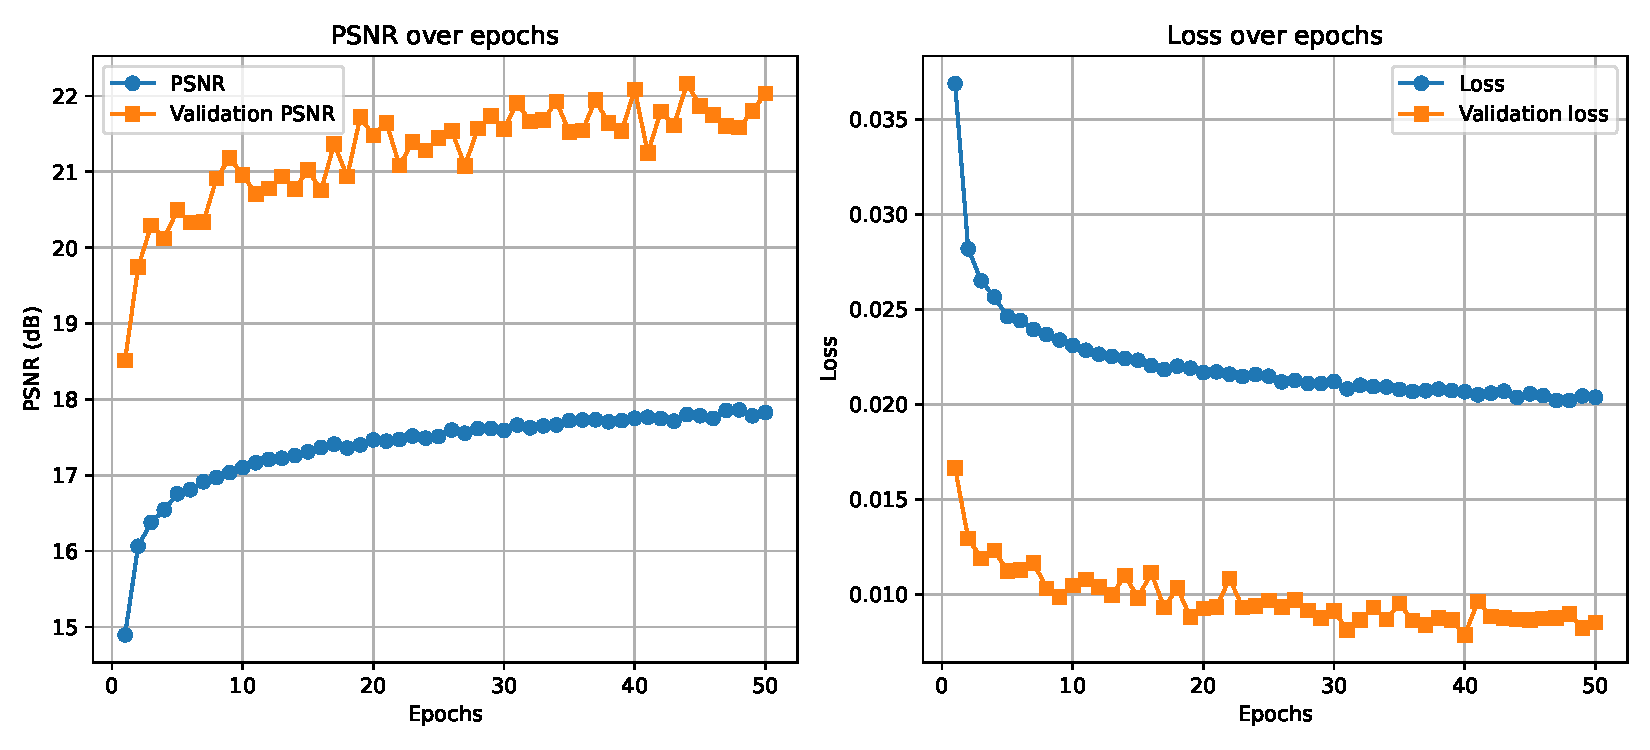
\includegraphics[width=\textwidth]{img/ch6/n2n_imagenet/psnr_loss_irfan.pdf}
        \caption{\acrshort{psnr} and loss curves for Irfan (Noise2Noise denoising).}
    \end{subfigure}
    
    \vspace{1cm}
    
    \begin{subfigure}{\textwidth}
        \centering
        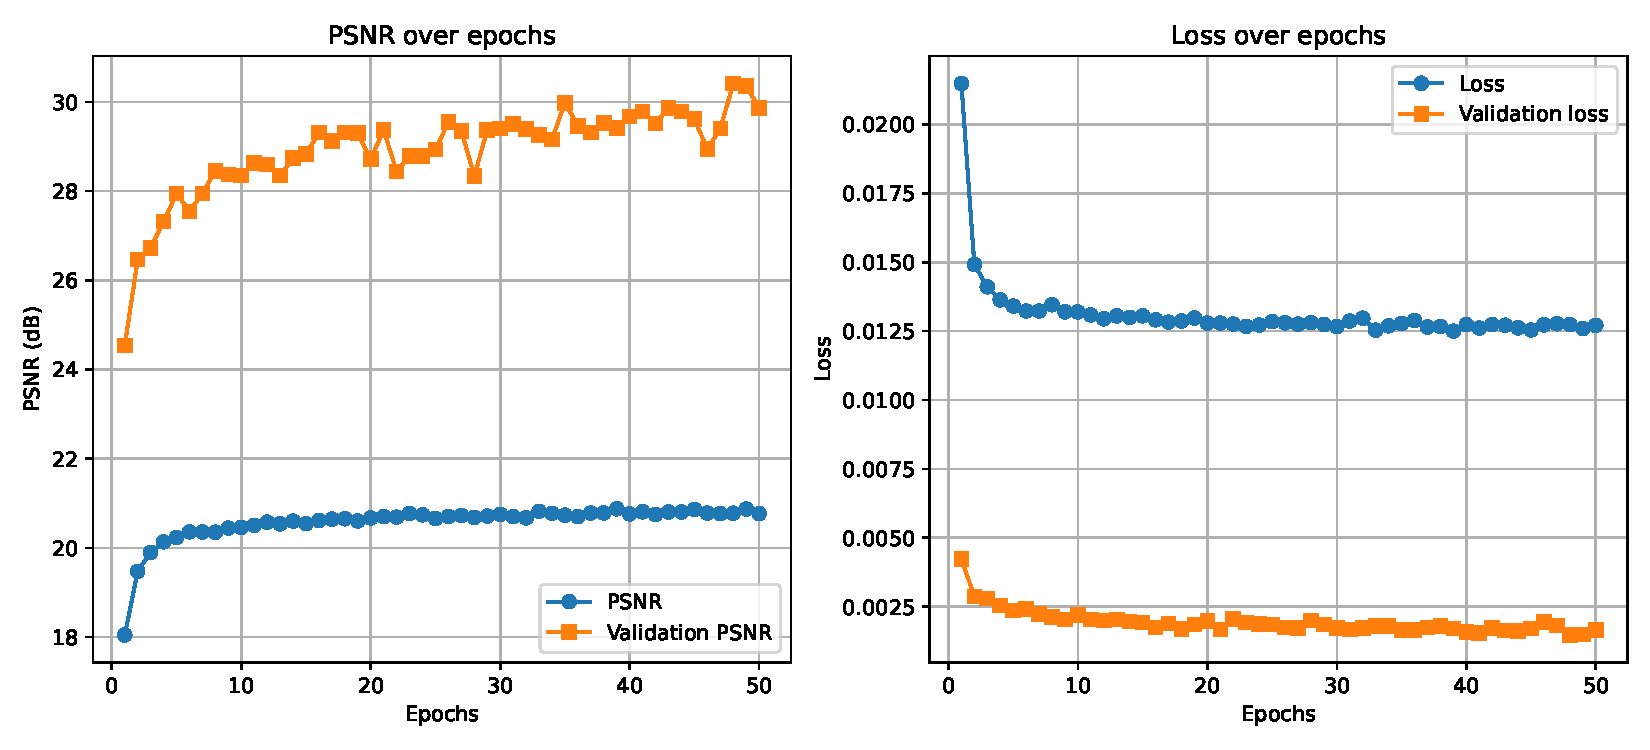
\includegraphics[width=\textwidth]{img/ch6/n2n_imagenet/psnr_loss_unet.pdf}
        \caption{\acrshort{psnr} and loss curves for U-Net (Noise2Noise denoising).}
    \end{subfigure}
    \caption{\acrshort{psnr} and loss curves for training the Noise2Noise model on (a) Irfan and (b) U-Net.}
    \label{fig:n2n-denoising-imagenet-curves}
\end{figure}


\subsubsection{Conclusion}
Overall, these results reaffirm the efficacy of the Noise2Noise methodology. The U-Net model, in particular, stands out for its ability to reconstruct fine image details, further validating its role as a robust solution for denoising tasks. Though these results set a strong foundation for applying Noise2Noise to spectrograms, challenges such as the absence of paired noisy spectrograms will require careful consideration.

\subsection{Part II: Transitioning to underwater acoustic spectrograms}

The previous section showed unequivocally that the Noise2Noise methodology works on natural images. We now turn our attention to the central question of this chapter: can Noise2Noise be effectively adapted to underwater acoustic spectrograms? 

While the Noise2Noise methodology has demonstrated its robustness in domains with clearly defined noise characteristics, the transition to underwater acoustics presents unique challenges. The technique relies on two key assumptions: having 1. paired data of the same event with 2. uncorrelated, zero-mean noise. In underwater acoustics, fulfilling these requirements is far from straightforward. The lack of public hydrophone array datasets limits our access to multiple recordings of the same event, and underwater noise often deviates from the strict zero-mean condition. 

The objective of this experiment is to explore whether these assumptions can be approximated. Instead of relying on hydrophone array recordings of the same event, we propose using spectrograms from the same vessel recorded at different times. By pairing spectrograms that share the same underlying signal but with varying noise, we aim to adapt the Noise2Noise framework to the complexities of underwater acoustic data. This experiment serves as an initial step in evaluating the feasibility of leveraging Noise2Noise for denoising tasks in this challenging and unexplored domain.

\subsubsection{Methodology}

To explore the application of Noise2Noise on underwater acoustic spectrograms, we began by identifying segments from the DeepShip dataset corresponding to vessels with multiple recordings. This step was necessary as the Noise2Noise framework relies on pairing spectrograms from the same vessel recorded at different times to approximate a shared underlying signal. Applying this filter reduced the dataset to 37,377 spectrograms.

The dataset was manually partitioned into training, validation, and testing sets in a 70-10-20 ratio. Care was taken to ensure that all recordings associated with a specific vessel were confined to the same split. This precaution was necessary to prevent scenarios where the algorithm would fail to find related spectrogram pairings for certain vessels, leading to errors during training.

% \begin{table}[htbp]
% \centering
% \caption{DeepShip train-validation-test split for approximating Noise2Noise by using related segments as inputs.}
% \label{tab:diff-spec-val-test-split}
% \begin{tabular}{lll}
% \toprule
% \textbf{Class} & \textbf{Validation Ships} & \textbf{Test Ships} \\ \midrule
% \multirow{3}{*}{Cargo}      & Anastasia & \multirow{2}{*}{Poyang 477669100} \\
%                             & Capricornus Leader & \\
%                             & Merlin Arrow & Seaspan Reliant \\ \midrule
% \multirow{6}{*}{Passengership}  & Mayne Queen & \multirow{6}{*}{Northern Adventure} \\
%                             & V2V Empress & \\
%                             & Safari Quest & \\
%                             & Salish Orca & \\
%                             & Salish Raven & \\
%                             & Seven Seas & \\ \midrule
% \multirow{10}{*}{Tanker}    & Cabo De & \multirow{10}{*}{Alfred N} \\
%                             & Champion Cornelia & \\
%                             & Champion Istra & \\
%                             & Navig8 Stellar & \\
%                             & Amagi Galaxy & \\
%                             & Argent Daisy & \\
%                             & Argent Sunrise & \\
%                             & Aristoklis & \\
%                             & Bochem London & \\
%                             & Caribbean Spirit & \\ \midrule
% \multirow{3}{*}{Tug}        & Ocean Betty & \multirow{3}{*}{Seaspan Eagle} \\
%                             & Seaspan Queen & \\
%                             & Sea Imp & \\ \bottomrule
% \end{tabular}
% \end{table}

We developed a custom data generator, \texttt{N2NDeepShipGenerator}, to streamline the pairing process. During initialisation, the generator precomputed all possible spectrogram pairings for efficiency. At runtime, it produced random pairs of spectrograms from the same vessel but from different recordings. This pairing ensured that the noise was uncorrelated while the underlying signal remained similar, approximating the core assumptions of the Noise2Noise framework.

Evaluating the models posed a unique challenge due to the lack of a clean ground truth, which precluded the use of conventional metrics like \acrshort{psnr}. Instead, we employed two alternative metrics: mean squared error loss and \acrshort{ssim}. While \acrshort{mse} quantified the overall reconstruction error, \acrshort{ssim} offered insight into how well the structural content of the spectrograms was preserved.

Both the Irfan and U-Net models were trained for 50 epochs each. While training to 150 epochs was ideal (as in the original Noise2Noise paper), computational limitations necessitated a shorter training duration. The training pipeline was implemented using TensorFlow, and all experiments were conducted on an Alienware laptop equipped with GPU acceleration to manage the computational demands of the large dataset.

\subsubsection{Results}

The results of this experiment, summarised in Table \ref{tab:n2n-diff-spec-results}, show the loss and \acrshort{ssim} metrics for the Irfan and U-Net models. Visual outputs from the models are presented in Figure \ref{fig:n2n-diff-spec-results}. Unfortunately, the experiment yielded underwhelming results, with both models achieving extremely low \acrshort{ssim} scores, indicating poor structural similarity between the input and output spectrograms.

In addition to poor performance metrics, the models failed to converge meaningfully during training. As seen in Figure \ref{fig:n2n-diff-spec-loss-curves-irfan}, the Irfan model's validation loss showed no downward trend, suggesting that the model struggled to learn any effective mappings. While the U-Net model demonstrated some convergence (Figure \ref{fig:n2n-diff-spec-loss-curves-unet}), the improvement in loss was minimal, decreasing by only 0.002 over 50 epochs. This lack of progress indicates significant challenges in adapting the Noise2Noise methodology to the underwater acoustic spectrogram dataset under the current experimental conditions.

\begin{table}[htbp] 
\centering 
\caption{Comparison of loss and \acrshort{ssim} values for the Irfan and U-Net models under the Noise2Noise approximation.} 
\label{tab:n2n-diff-spec-results} 
    \begin{tabular}{lcc} 
    \toprule 
    \textbf{Model} & \textbf{Loss} & \textbf{\acrshort{ssim}}\\ \midrule 
    Irfan & $2.12 \times 10^{-2}$ & 0.118 \\
    U-Net & $1.77 \times 10^{-2}$ & 0.129 \\
    \bottomrule
    \end{tabular} 
\end{table}

\begin{figure}[p]
    \centering
    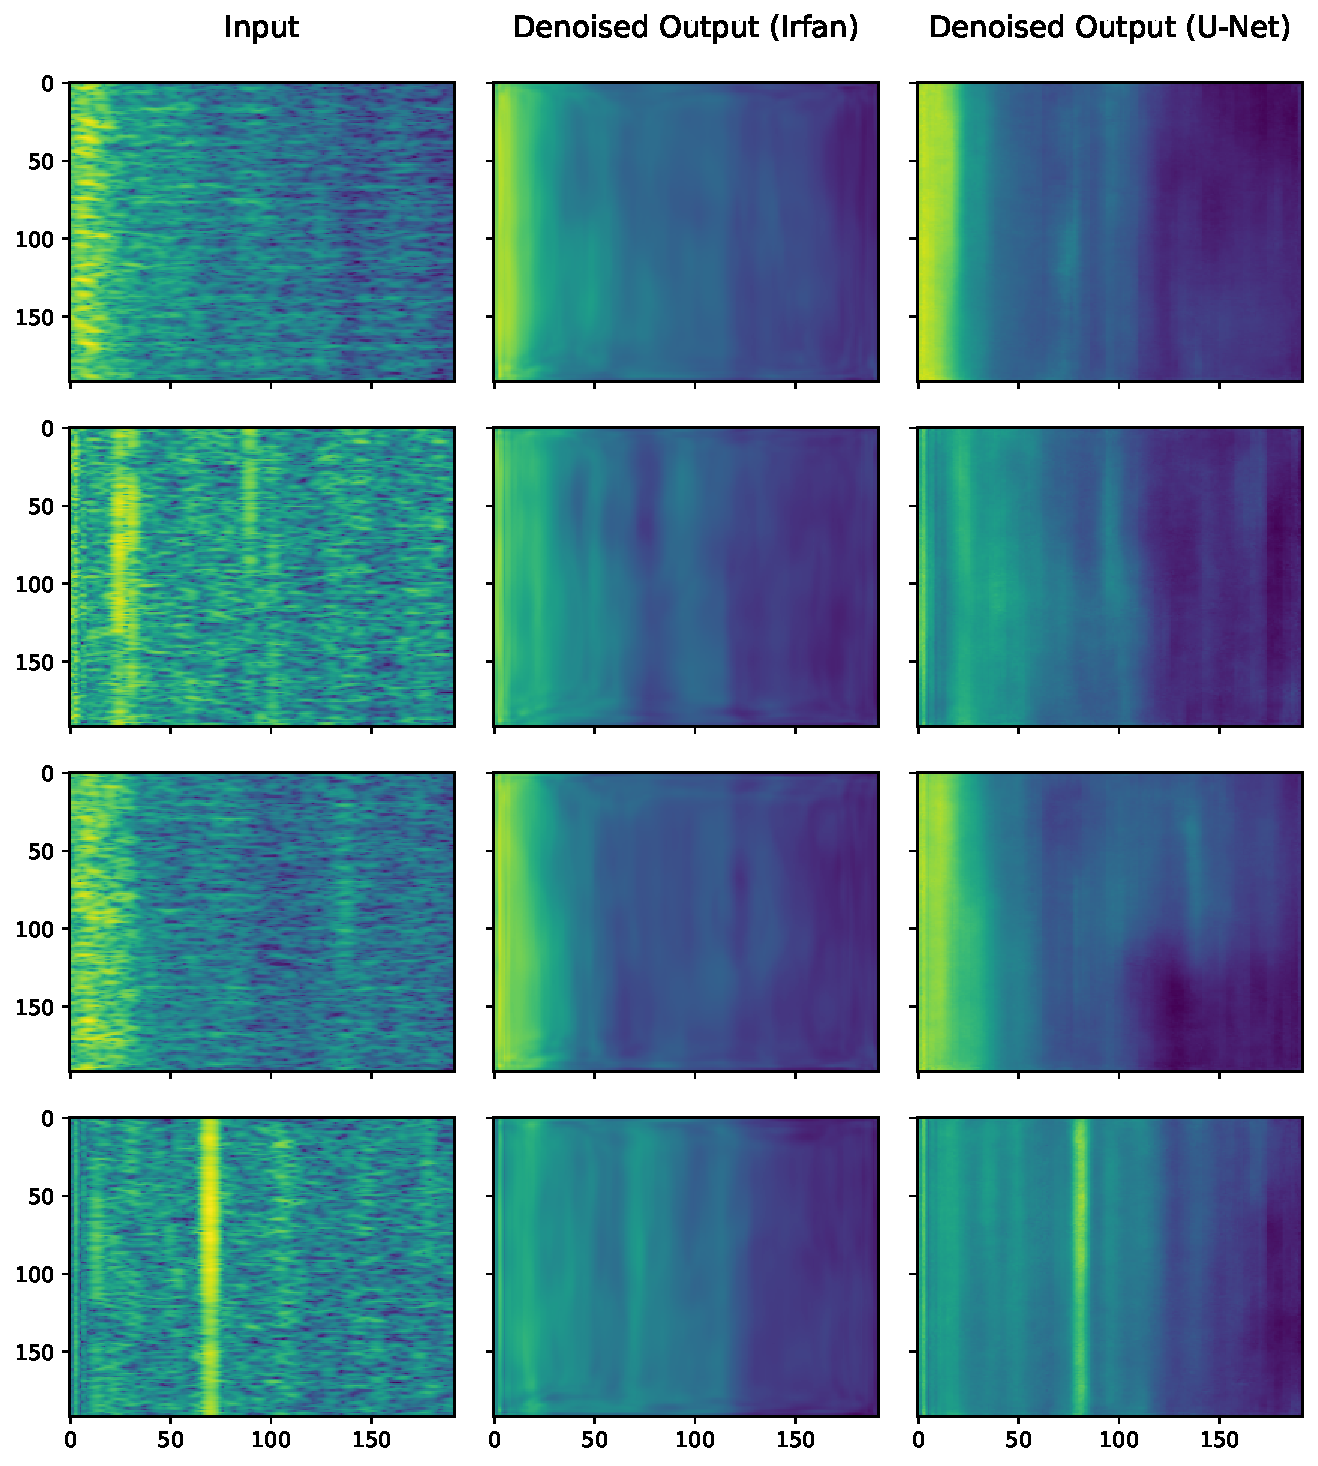
\includegraphics[width=\textwidth]{img/ch6/in_neq_out/results.pdf}
    \caption{Outputs generated by the Irfan and U-Net models for the Noise2Noise experiment on spectrograms. The visualisations reveal heavily blurred and smoothed spectrograms that fail to retain key features from the original input.}
    \label{fig:n2n-diff-spec-results}
\end{figure}

\begin{figure}[p]
    \begin{subfigure}{\textwidth}
        \centering
        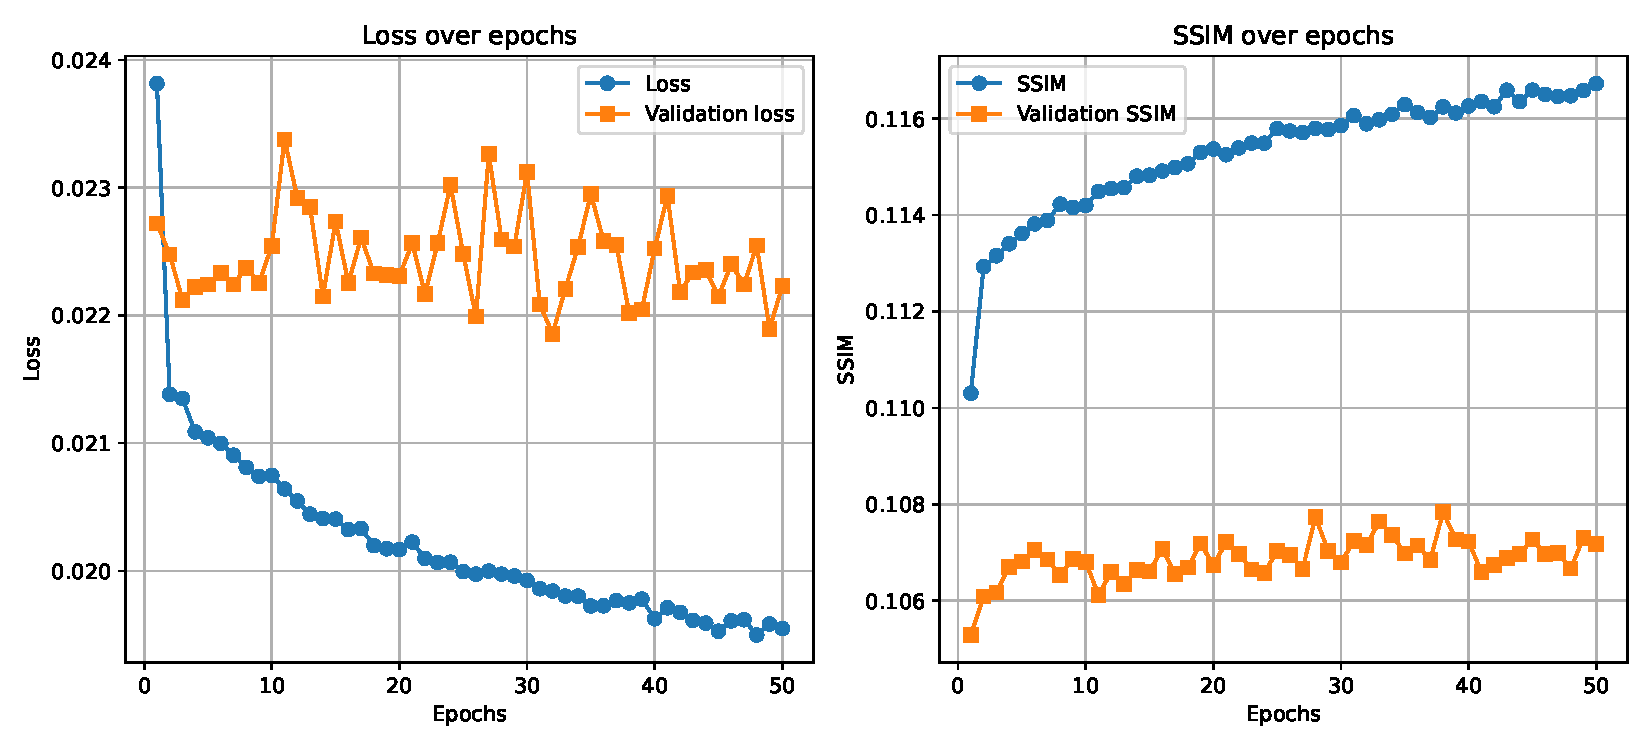
\includegraphics[width=\textwidth]{img/ch6/in_neq_out/irfan/loss_ssim_curves.pdf}
        \caption{Loss and \acrshort{ssim} curves for the Irfan model.}
        \label{fig:n2n-diff-spec-loss-curves-irfan}
    \end{subfigure}

    \vspace{0.5cm}

    \begin{subfigure}{\textwidth}
        \centering
        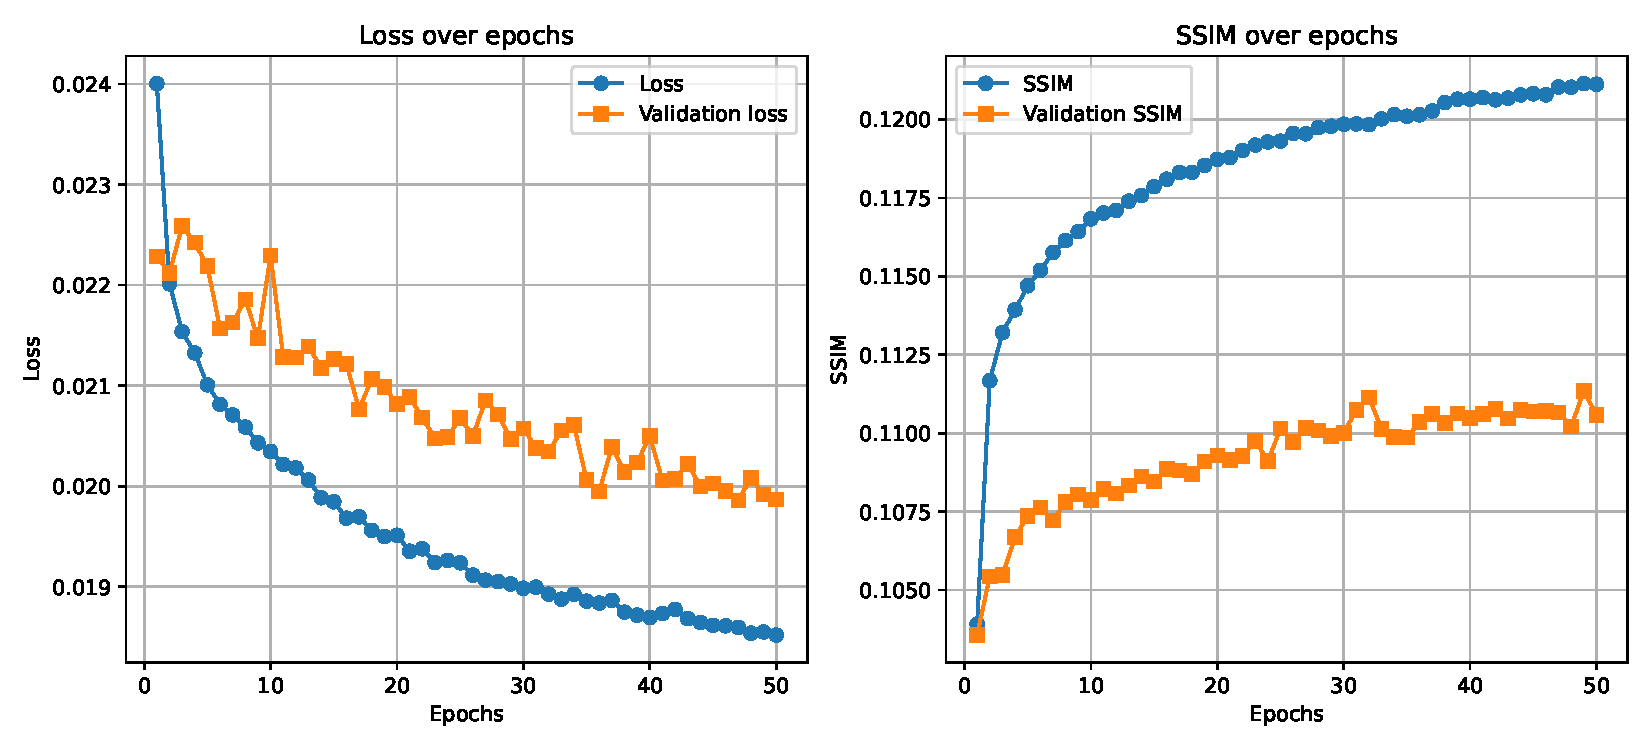
\includegraphics[width=\textwidth]{img/ch6/in_neq_out/unet/loss_ssim_curves.pdf}
        \caption{Loss and \acrshort{ssim} curves for the U-Net model.}
        \label{fig:n2n-diff-spec-loss-curves-unet}
    \end{subfigure}
    \label{fig:n2n-diff-spec-loss-curves}
    \caption{Loss and \acrshort{ssim} curves for attempting to approximate Noise2Noise denoising principles on spectrogram data.}
\end{figure}

\subsubsection{Discussion}
The visualised outputs (Figure \ref{fig:n2n-diff-spec-results}) reveal the core problem: both the Irfan and U-Net models produced blurred and overly smoothed spectrograms, failing to preserve key features of the input. Despite the U-Net slightly outperforming the Irfan model in terms of loss and \acrshort{ssim}, neither model succeeded in creating outputs that could be considered meaningful or useful for downstream tasks.

These results make it clear that the Noise2Noise framework is highly reliant on its assumptions: the input-output pairs must share the same underlying signal but have independent noise distributions. In the context of this experiment, these conditions were only approximated by pairing spectrograms from the same vessel recorded on different days. However, underwater noise is highly dynamic, influenced by environmental factors such as weather, water currents, and background biological activity. These factors likely introduced significant discrepancies in the noise distributions of the paired spectrograms, undermining the Noise2Noise methodology's core premise. Without truly independent noise distributions and a shared signal, the models struggled to identify and learn meaningful patterns.

The poor performance metrics and lack of convergence observed in this experiment strongly suggest that the current dataset and pairing strategy are inadequate for successfully applying Noise2Noise to underwater acoustic spectrograms. To address these challenges, future work should focus on improving pairing strategies, ideally through collecting hydrophone array data to provide multiple recordings of the same event with truly independent noise distributions. This would align more closely with the Noise2Noise framework.

\subsubsection{Conclusion}

This experiment highlights the significant challenges of adapting the Noise2Noise framework to underwater acoustic spectrograms. Despite its success in other domains, the methodology struggled under the constraints of this experiment, yielding outputs that failed to preserve meaningful spectrogram features. The core issue lies in the inability to satisfy the Noise2Noise assumptions: the paired spectrograms did not share identical underlying signals with independent noise distributions, as environmental factors such as weather and biological activity introduced substantial variability in the noise conditions between recordings.

Although the experiment was unsuccessful, it underscores the importance of developing more robust pairing strategies and dataset collection techniques, such as leveraging hydrophone arrays to capture multiple recordings of the same event with minimal noise variability. Ultimately, these insights provide a foundation for future research aimed at refining the application of Noise2Noise principles to underwater acoustic data.

\section{Experiment 2: Masking-based denoising}

This experiment evaluates the effectiveness of masking-based denoising for underwater acoustic spectrograms, specifically using the DeepShip dataset. The objective is to develop a deep learning model capable of accurately segmenting narrowband events from spectrograms while effectively removing noise. Additionally, the experiment explores the potential of automatic masking techniques to enhance the segmentation process.

\subsection{Methodology}

The development of an image segmentation model to extract narrowband events from spectrograms required both the original spectrogram images and their corresponding ground-truth masks. Ground-truth masks are essential for training as they highlight regions of interest within the spectrograms, providing the model with guidance on what to focus on during training.

The original spectrogram images were generated using the custom \texttt{wavToSpec()} function, described in Section \ref{sec:inputs}, which includes the capability to export spectrograms in \texttt{.png} format.

The primary challenge lay in the creation of ground-truth masks, as the DeepShip dataset does not include pre-existing labelled data. This limitation stems from the niche nature of the dataset and the field of underwater acoustic research, compounded by the labour-intensive and expertise-dependent nature of spectrogram annotation. Unlike conventional image labelling tasks, annotating spectrograms requires domain-specific knowledge to accurately identify features of interest, such as vessel-related narrowband tracks. Furthermore, the labelling process is sensitive to the specific spectrogram parameters and export configurations used, adding an additional layer of complexity. Consequently, the generation of ground-truth masks necessitated either manual labelling or the use of an automated masking algorithm.

Manual labelling was chosen for the purposes of this experiment. Using MATLAB's \textit{Image Labeler} application, a total of 356 spectrograms were manually labelled to highlight narrowband frequencies and tracks of interest (Figure \ref{fig:matlab-image-labeller}). This process was quite labour-intensive, requiring careful annotation of each spectrogram. To facilitate model training, custom MATLAB functions were developed to convert the proprietary mask format produced by the \textit{Image Labeler} into binary masks. In this format, the background is represented by pixel values of 0, while the regions of interest are represented by pixel values of 255 (Figure \ref{fig:matlab-image-labeller-result}).

The final dataset, consisting of 356 spectrograms and their corresponding binary masks, was divided into an 80-20 train-test split. These data splits were processed using a custom \texttt{ImageSegmentationGenerator} to create batches of spectrograms and their associated masks for model training. The U-Net architecture, a well-established framework for image segmentation tasks (Section \ref{subsec:unet}), was employed as the segmentation model. The model was compiled using the Adam optimiser with a learning rate of $10^{-5}$, and binary cross-entropy was utilised as the loss function. Model performance was evaluated using binary accuracy and the binary \acrfull{iou} metric.

\begin{figure}
    \begin{subfigure}{\textwidth}
        \centering
        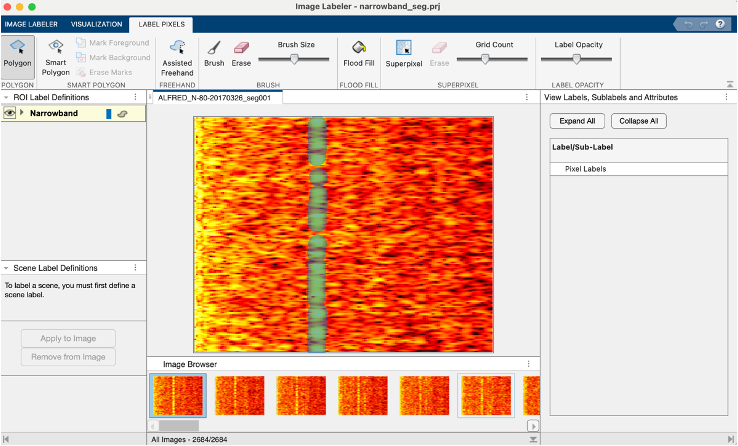
\includegraphics[width=\textwidth]{img/ch6/masking/matlab_image_labeller.png}
        \caption{The \textit{Image Labeler} program is used to manually annotate the region of interest in the spectrogram, with the mask highlighted in light blue.}
        \label{fig:matlab-image-labeller}
    \end{subfigure}
    
    \vspace{1cm}
    
    \begin{subfigure}{\textwidth}
        \centering
        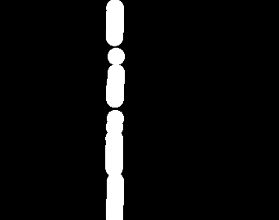
\includegraphics[width=0.5\textwidth]{img/ch6/masking/binary_mask_ex.png}
        \caption{The binary mask output corresponding to the spectrogram in subfigure (a). The mask is a binary image, where the background is represented by 0, and the region of interest is represented by 255.}
        \label{fig:matlab-image-labeller-result}
    \end{subfigure}
    \caption{The image masking process using MATLAB's \textit{Image Labeler}.}
    \label{}
\end{figure}

\subsection{Results}

The model was trained for 500 epochs, and the results were evaluated on the test set. The performance metrics yielded an overall loss of 38.27\%, binary accuracy of 93.97\%, and binary \acrshort{iou} of 0.49. Figure \ref{fig:unet-segmentation-results} provides a visual comparison of the original spectrograms, the ground-truth masks, and the masks predicted by the U-Net model.

\begin{figure}[p]
    \centering
    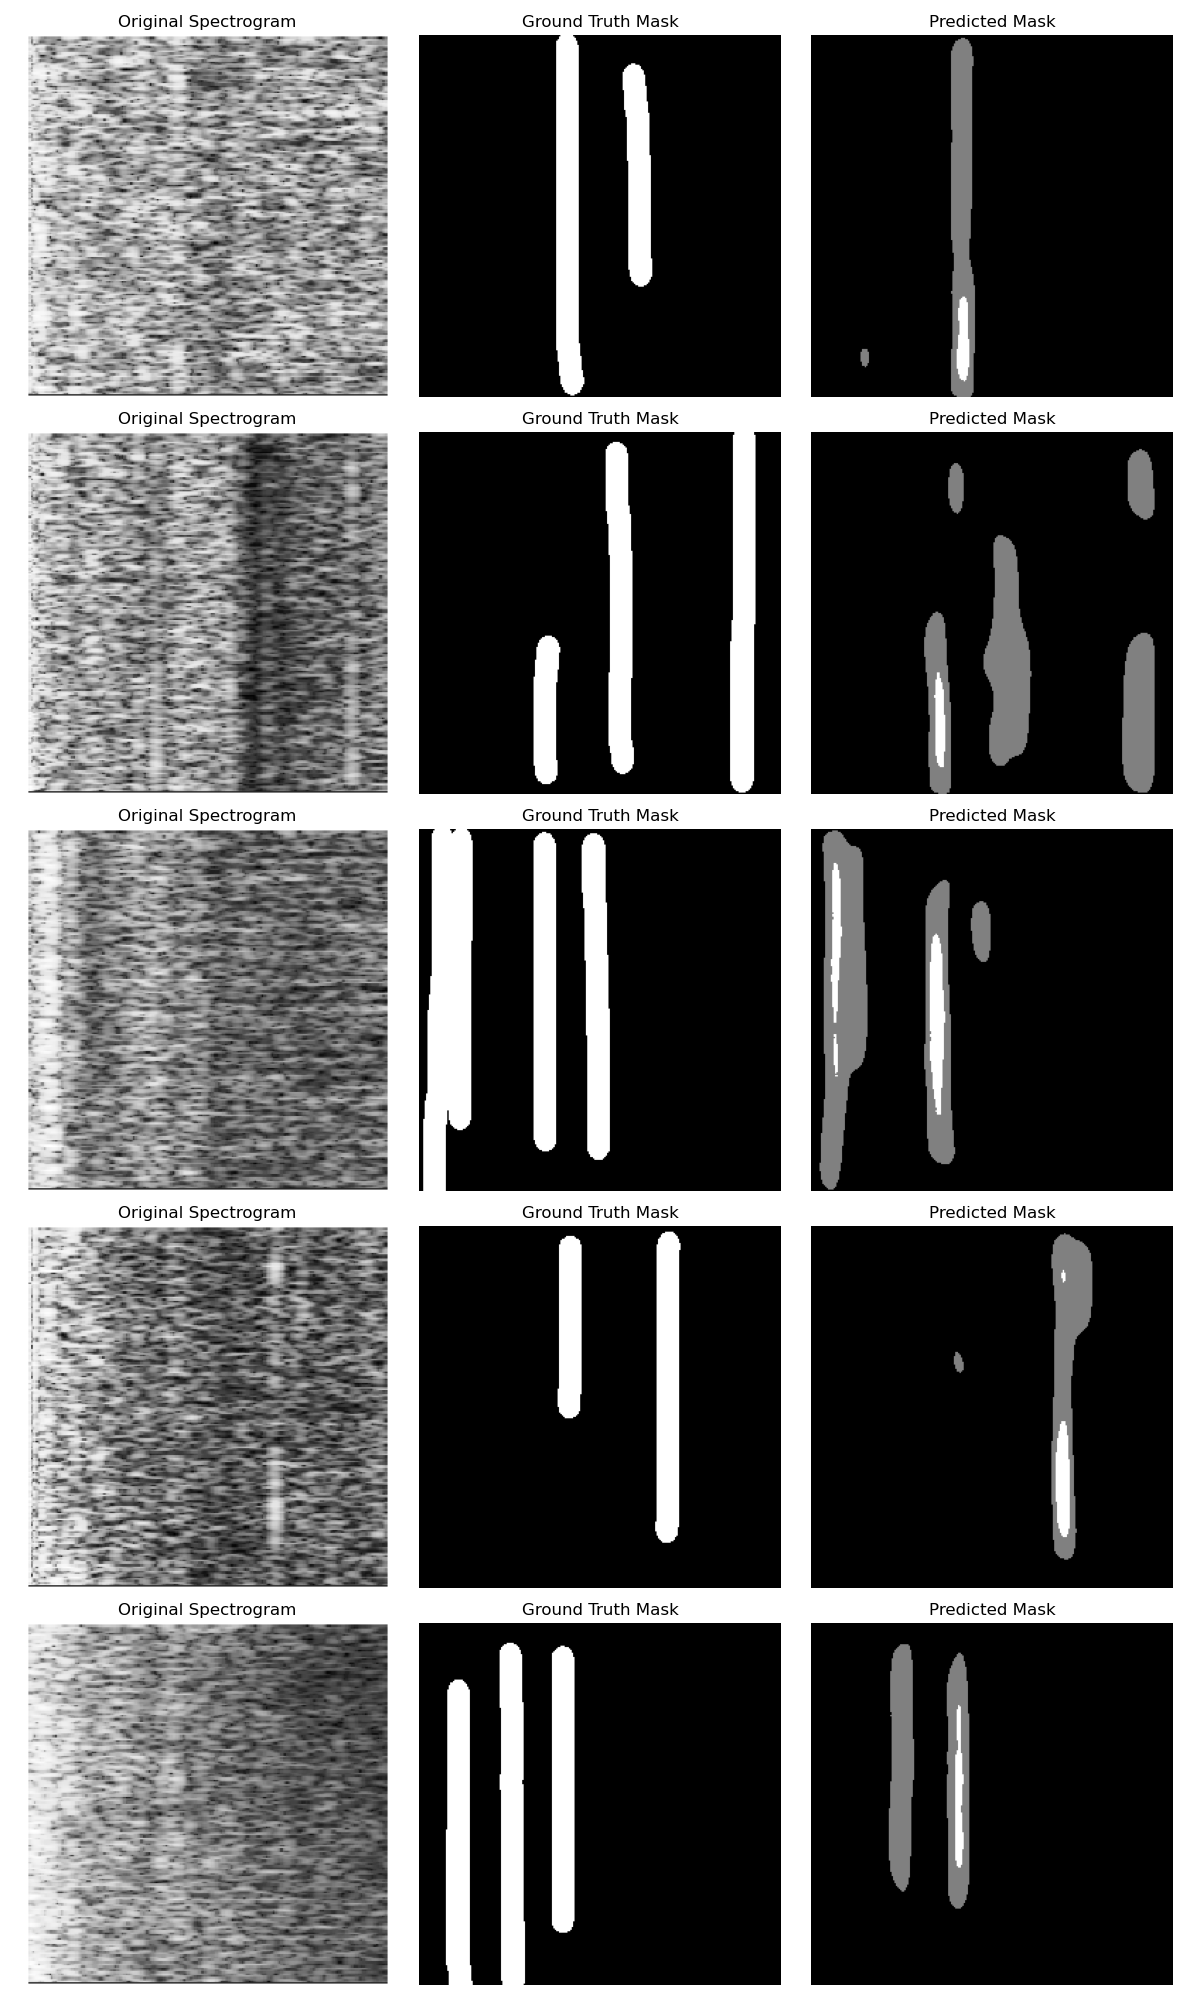
\includegraphics[width=0.8\textwidth]{img/ch6/masking/unet_segmentation_500_epochs.png}
    \caption{Comparison of original spectrograms, ground truth masks, and predicted masks after the U-Net model was trained for 500 epochs.}
    \label{fig:unet-segmentation-results}
\end{figure}

\subsection{Discussion}
The results of the U-Net model, with a binary accuracy of 93.97\% and a relatively low binary \acrshort{iou} score of 0.49, suggest that the predicted masks were effective at identifying many narrowband events but fell short of capturing all instances. As illustrated in Figure \ref{fig:unet-segmentation-results}, the model often identified regions of interest with reasonable accuracy, but some events were missed entirely, and random artifacts occasionally appeared in areas where they were not expected.

One major challenge in this experiment was the resolution of the spectrograms. The \acrshort{fft} length of 1024, as specified in Table \ref{tab:powerspectrogram-parameters}, may have provided insufficient frequency resolution to clearly represent narrowband events. The low resolution made it difficult for the model to distinguish these events from the surrounding noise, resulting in less precise masks. This reinforces the importance of high-quality input data for effective model training -- in other words: ``garbage in, garbage out.''

Another contributing factor was the quality of the ground-truth labels. Manual annotation was conducted by myself, a student of software engineering, rather than a domain expert in sonar processing. While this may have been sufficient for preliminary experimentation, annotations made by a skilled sonar technician would be more precise, especially with higher-resolution spectrograms. Improved ground-truth labels would provide the model with better guidance during training, potentially leading to more accurate segmentation outcomes.

Additionally, the dataset size -- 356 annotated spectrograms -- was a major limiting factor in this experiment. This data volume is far below the scale of datasets typically used for state-of-the-art image segmentation models, which often consist of tens of thousands of images. While the limited dataset was sufficient for initial experimentation, future work should aim to increase the number of annotated samples to at least a few thousand to improve model generalisation and robustness.

For future work, several promising avenues could be pursued. First, improvements in both the input data (higher-resolution spectrograms) and the labelling process (expert-provided masks) could address many of the challenges observed in this experiment. Secondly, the use of automatic masking techniques presents an exciting opportunity to overcome the time, cost, and expertise constraints associated with manual labelling. Two promising methods in this area are the HIDE \& SEEK algorithm and track detection algorithms.

The HIDE \& SEEK algorithm, developed by Akeret et al. in 2017 \cite{akeret_hide_2017}, consists of two related Python packages designed for simulating and processing radio survey data. The SEEK package, in particular, removes artifacts from radio-frequency interference (RFI) and generates masks identifying these interference areas. Although RFI and noise in underwater acoustic data differ in nature, they share common characteristics, and SEEK has shown promising results when applied to audio data. Initial results from applying SEEK to DeepShip spectrograms (Figure \ref{fig:seek-output}) are encouraging, though further refinement and testing are required to optimise this approach -- work that could not be fully explored within the time constraints of this project.

\begin{figure}[htbp]
    \centering
    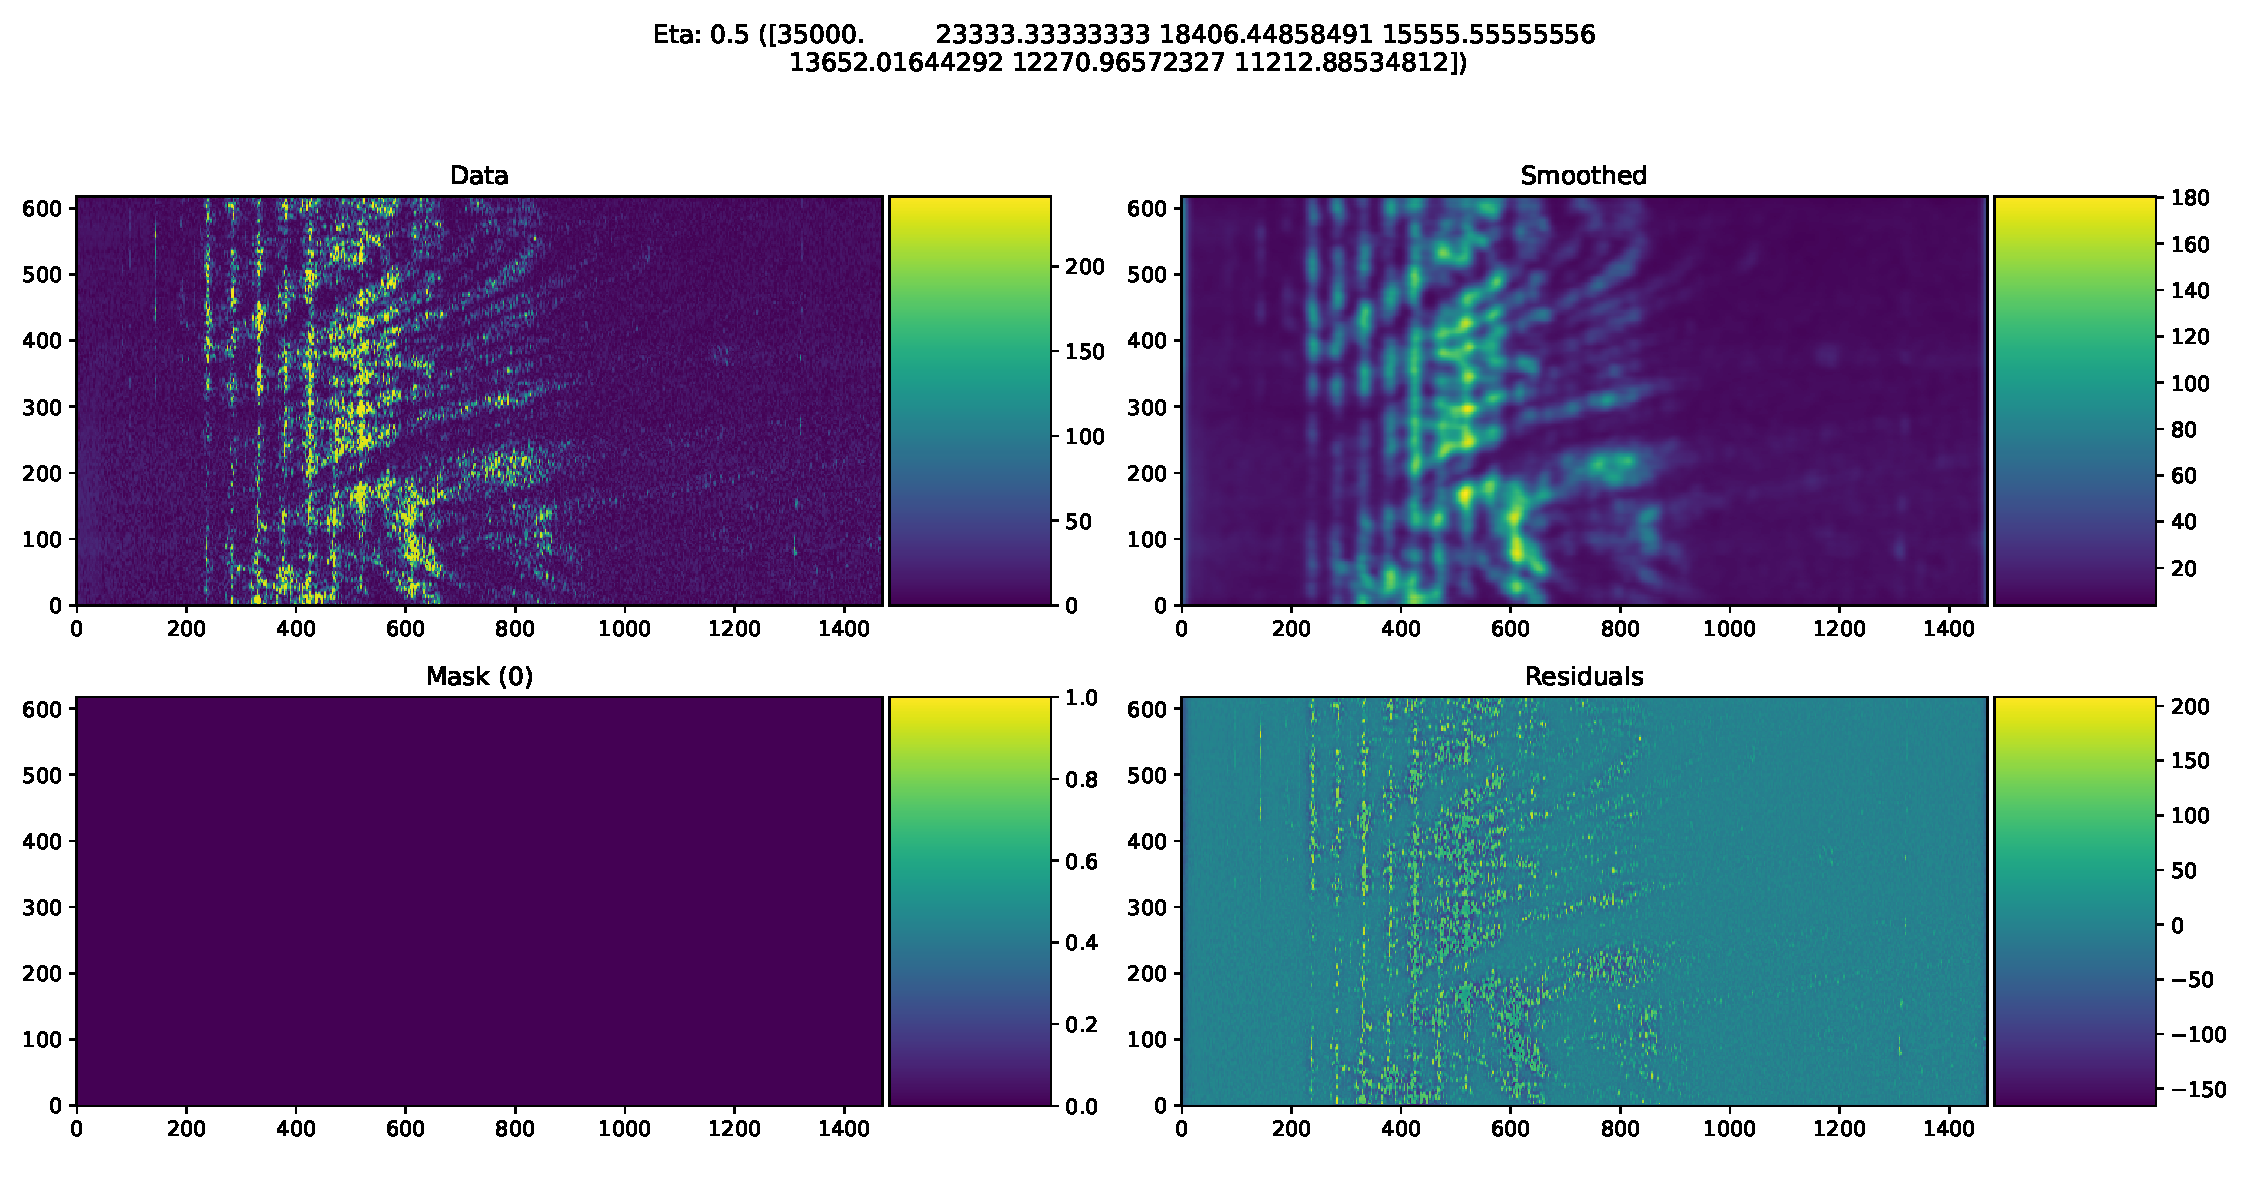
\includegraphics[trim={0 0 0 2cm},clip,width=\linewidth]{img/ch6/masking/seek_output.pdf}
    \caption{Preliminary results from applying the SEEK algorithm to spectrograms. The output shows the potential of SEEK for identifying regions of interest in spectrograms, although further fine-tuning is required.}
    \label{fig:seek-output}
\end{figure}

The second promising direction lies in exploring track detection algorithms. These algorithms are specifically designed to detect narrowband tracks in spectrograms, which makes them highly relevant to this task. A brief review of track detection algorithms was presented earlier in Table \ref{tab:track-detection-review}. These algorithms could provide a means of approximating ground-truth masks without manual intervention. Leveraging these algorithms could significantly accelerate the data preparation process while maintaining a high standard of accuracy.

Finally, a key limitation of this study was the absence of an evaluation step that applied the generated masks to the baseline \acrshort{cnnlstm} model to assess their impact on classification performance. Conducting such an evaluation would offer valuable insights into the practical utility of masking-based denoising techniques for underwater acoustic target recognition tasks. Future research should prioritise this step to fully explore the potential of these approaches.

\subsection{Conclusion}

The U-Net model demonstrated strong potential for identifying key narrowband events in spectrograms, achieving a binary accuracy of 93.97\%. However, the relatively low binary \acrshort{iou} score of 0.49 underscores the need for improvements in mask precision and the detection of all narrowband events. These findings suggest that the resolution of the spectrograms and the quality of the manual labelling process played critical roles in limiting the model's performance. Future efforts should prioritise the use of higher-resolution spectrograms and expert-provided ground-truth annotations to ensure that the regions of interest are accurately captured. Expanding the dataset size is also recommended to enhance model generalisation and robustness.

Furthermore, the exploration of automatic masking techniques offers a promising path forward. Algorithms like HIDE \& SEEK and track detection methods could significantly reduce the time and effort required for manual annotation while maintaining accuracy. Preliminary results using SEEK were encouraging, though additional refinement and testing are needed to optimise its application to underwater acoustic data. By combining improved input data with advanced automatic masking techniques, future research could produce more accurate segmentation masks in the aim of enhancing classification performance in underwater acoustic target recognition tasks.

\section{Concluding remarks}

The challenges of denoising underwater acoustic signals underscore the complexities of adapting machine learning techniques originally designed for image data to a vastly different domain. In the realm of images, noise predominantly arises from the sensor itself -- random fluctuations inherent to the image capture process. In contrast, noise in underwater signals stems from a multitude of external sources, including marine wildlife, ship traffic, industrial activity, and environmental factors like waves and water currents. This fundamental difference is likely a key reason why our first experiment, applying the Noise2Noise framework to spectrograms, failed to produce meaningful results. Techniques developed for reducing sensor noise are ill-suited to address the diverse and dynamic noise conditions present in underwater environments.

Noise2Noise, while highly effective for image denoising, relies on specific assumptions; namely, that paired inputs share the same underlying signal but have uncorrelated noise. These assumptions are difficult to replicate in underwater acoustics, where the noise is influenced by countless variables that can change over time and space. The experiment highlighted the limitations of current approaches in adapting image-based methodologies to the underwater domain, particularly when paired data is unavailable or when noise characteristics deviate significantly from the assumptions underpinning these frameworks.

On the other hand, the masking-based approach presents a promising alternative for underwater signal denoising. By focusing on isolating regions of interest in spectrograms, the masking method bypasses some of the challenges associated with directly modeling noise. While the results of our masking experiments were not definitive, they indicate potential for future development. Continued exploration into automatic masking techniques, such as integrating advanced track detection algorithms or refining U-Net-based segmentation methods, could lead to significant advancements in underwater acoustic signal processing.

Ultimately, our findings reaffirm the dominance of traditional signal processing methods in underwater acoustics. Machine learning approaches, while transformative in other fields, must be tailored more carefully to the unique characteristics of this domain. The masking method offers a glimmer of hope for achieving this adaptation, and future work should focus on combining the strengths of signal processing with the adaptability of machine learning. By bridging these two paradigms, the potential for enhancing underwater acoustic signal classification and denoising could finally be realised.

\subsection{Future work}

In addition to the core work presented here, several other avenues of exploration were considered for this chapter but ultimately not pursued due to time constraints. One of the most promising of these avenues was the use of the \acrfull{n2v} algorithm for denoising underwater acoustic spectrograms.

The Noise2Noise framework, as demonstrated in Section \ref{subsec:recreating-n2n}, is highly effective at performing denoising without the need for clean target images. However, it has a major limitation: it requires paired noisy images with independent noise distributions for the algorithm to work. This dependency on paired data makes the approach less applicable in scenarios where only noisy data is available. Seeing as this is the case for most real-world applications -- including our own with underwater acoustic data -- the Noise2Noise framework may be more theoretically impressive than practical.

The Noise2Void algorithm, a successor to Noise2Noise, addresses this limitation by employing a truly self-supervised approach \cite{krull_noise2void_2019}. Unlike Noise2Noise, which relies on the properties of paired noisy images, Noise2Void exploits the inherent structure within the image itself to perform denoising. Specifically, the algorithm operates on the assumption that \textit{signal has structure and noise does not}. In practice, this means that the algorithm can predict the true signal for a given pixel by examining its surrounding context, while it is unable to predict the noise, which lacks a structured pattern. To achieve this, Noise2Void uses a technique known as \textit{blind spot learning}, where one pixel is excluded from the input image (the ``blind spot'') and the algorithm attempts to predict its value based on the surrounding pixels.

This method has demonstrated significant promise in the literature and has been successfully applied to various problems, though mostly related to medical imaging \cite{ashwini_denoising_2023, liu_lightweight_2022, kojima_denoising_2022, song_noise2void_2021, song_noise2void_2020}. Many improved versions of N2V have been published, and work on blind spot networks is still an open research area \cite{krull_probabilistic_2019, laine_high-quality_2019, hock_n2v2_2022, zhang_unleashing_2024}. Given its potential, we aimed to investigate its application to the domain of underwater acoustic signal processing, specifically for denoising spectrograms.

To explore this, we implemented the Noise2Void algorithm in Keras and trained it for 100 epochs, using the BSD training set for training and the BSD test set for validation. The denoising results on the BSD dataset, shown in Figure \ref{fig:n2v-results-natural}, qualitatively indicate that our implementation of Noise2Void produced quite accurate denoising results, which look visually comparable to those of both supervised methods and the Noise2Noise framework.

However, when we applied the algorithm to the DeepShip spectrograms, the results were suboptimal. As shown in Figure \ref{fig:n2v-results-specs}, the denoised spectrograms exhibited poor quality, and overall simply achieved a mild blurring effect. Upon further investigation, we determined that these issues were primarily due to issues in our implementation and mismatches in the input size, which were not adequately addressed within the time frame of this thesis.

With further refinement of the algorithm implementation, the Noise2Void algorithm could be successfully applied to the task of denoising underwater acoustic spectrograms, and could be a real, practically-applicable model for underwater acoustic signal denoising given that it only relies on single noisy image inputs.


\begin{figure}[p]
    \centering
    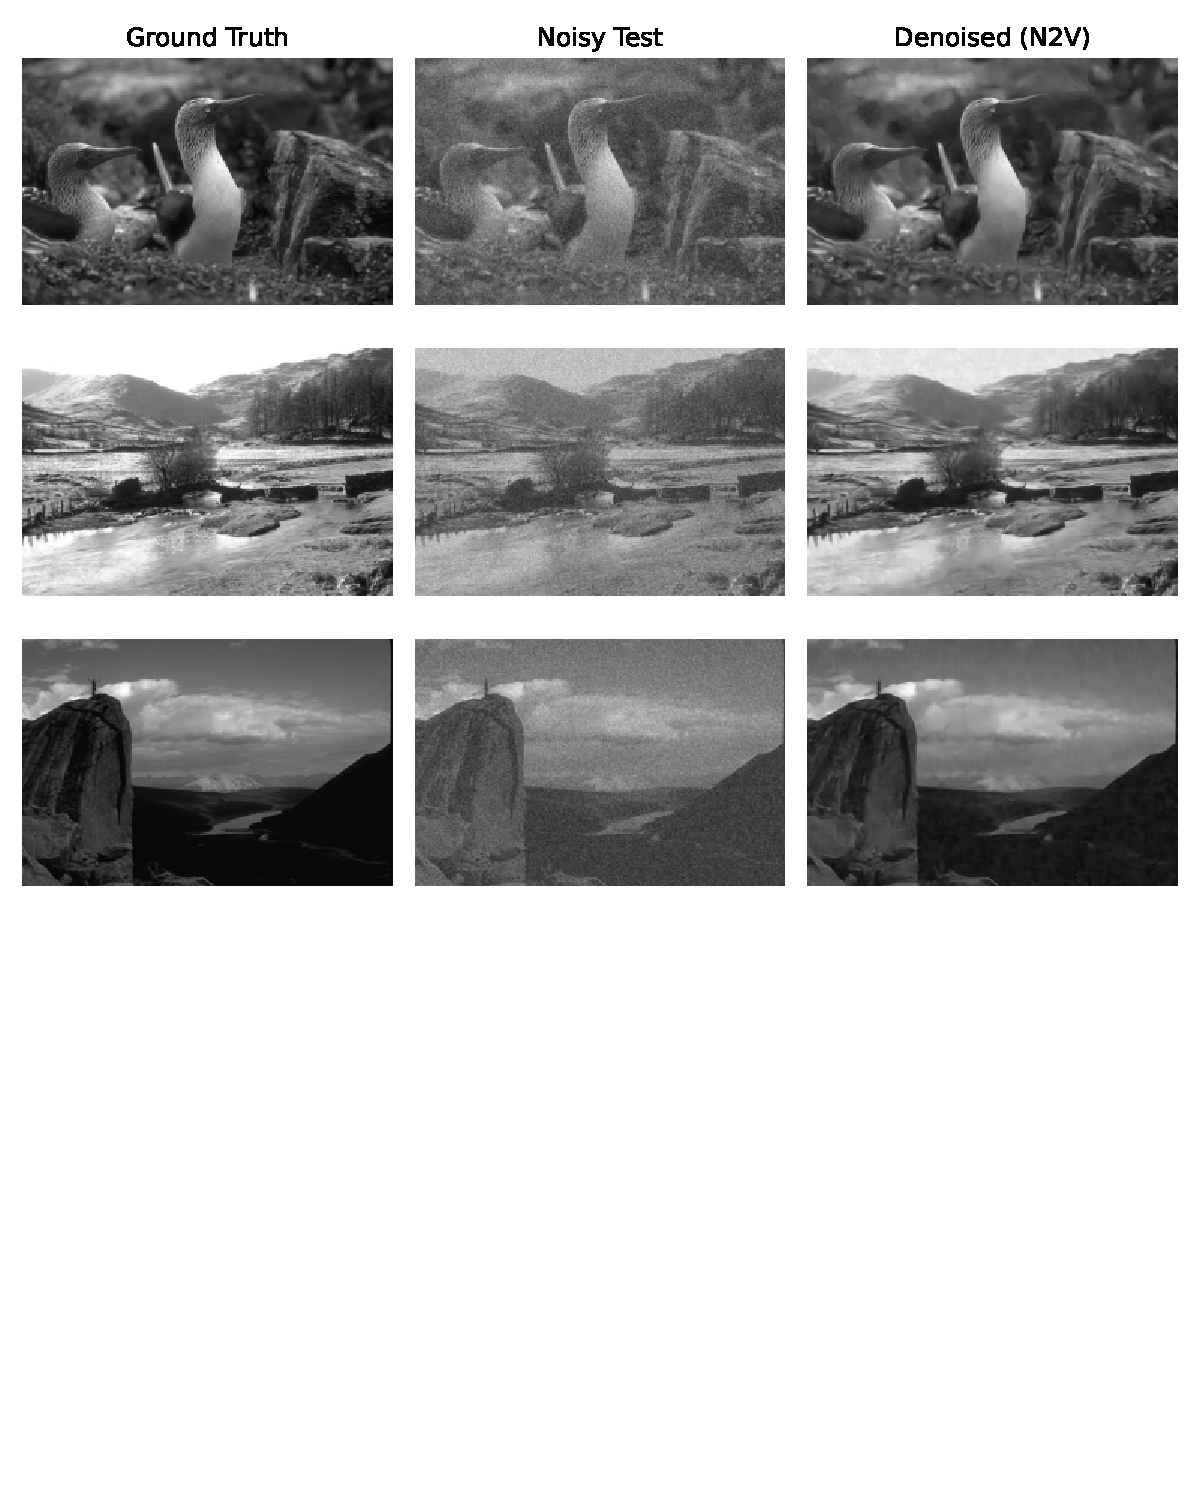
\includegraphics[trim={0.5cm 10cm 0.5cm 0},clip,width=\linewidth]{img/ch6/future_work/n2v_comparison_bsd.pdf}
    \caption{Denoising results on the BSD dataset using the Noise2Void algorithm.}
    \label{fig:n2v-results-natural}
\end{figure}

\begin{figure}[p]
    \centering
    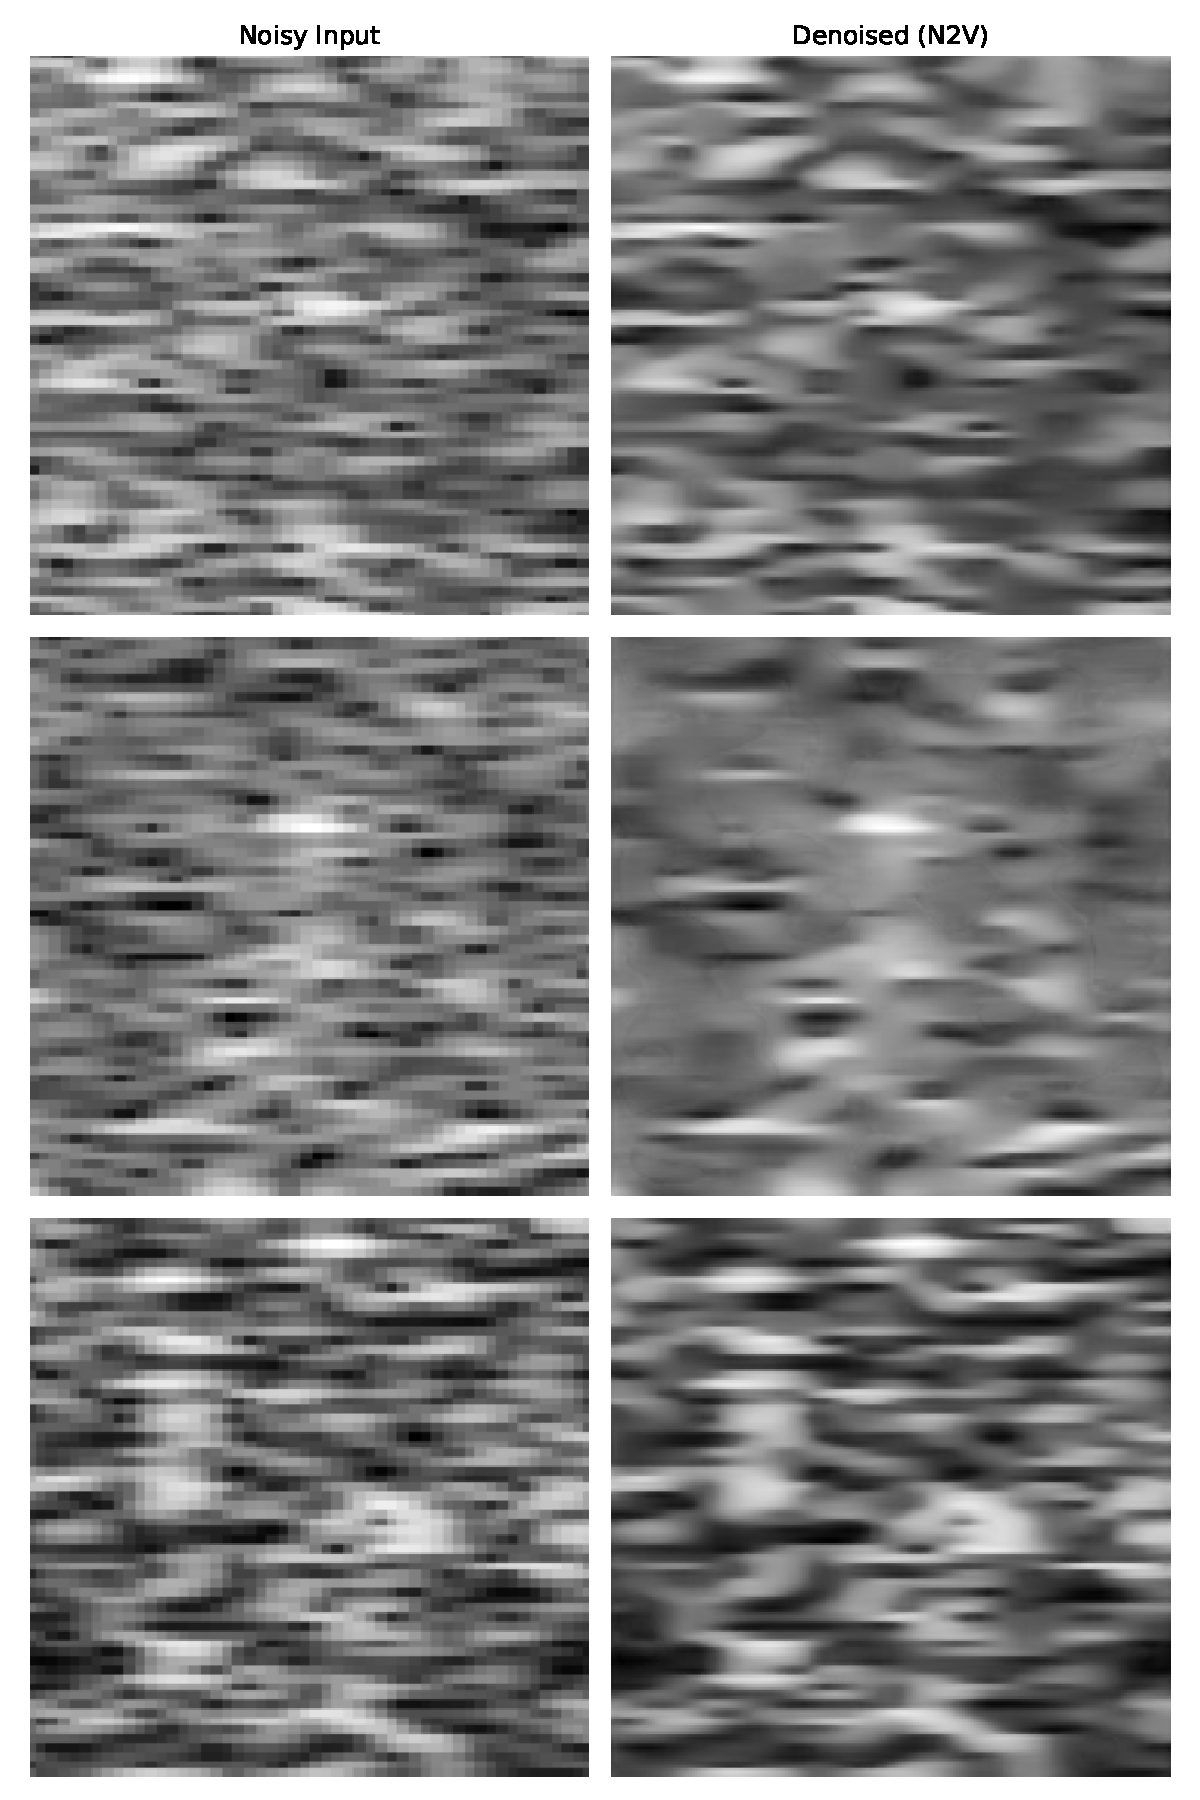
\includegraphics[width=0.7\linewidth]{img/ch6/future_work/n2v_comparison_specs.pdf}
    \caption{Denoising results on the DeepShip spectrograms using the Noise2Void algorithm. The poor results are attributed to challenges with the input size and algorithm implementation, which were not resolved within the scope of this thesis.}
    \label{fig:n2v-results-specs}
\end{figure}



